% ============================================================
% DATATHON 2026 — The Gridbreakers
% NeurIPS-style Report (4 pages + references/appendix)
% ============================================================
\documentclass{article}

% --- NeurIPS 2025 compatible packages ---
\usepackage[utf8]{inputenc}
\usepackage[T5]{fontenc}
\usepackage[vietnamese,english]{babel}
\usepackage{times}  % NeurIPS uses Times font

% NeurIPS page layout (replicate official margins)
\usepackage[a4paper, left=1.5in, right=1.5in, top=1in, bottom=1in]{geometry}
\usepackage[numbers]{natbib}
\usepackage{setspace}

% Graphics and tables
\usepackage{graphicx}
\usepackage{booktabs}
\usepackage{float}
\usepackage{caption}
\usepackage{subcaption}
\usepackage{multirow}
\usepackage{array}
\usepackage[usenames,dvipsnames]{xcolor}

% Math and code
\usepackage{amsmath}
\usepackage{amsfonts}
\usepackage{amssymb}
\usepackage[colorlinks=true,linkcolor=blue,citecolor=blue,urlcolor=blue]{hyperref}

% --- Compact spacing for 4-page limit ---
\setlength{\parskip}{3pt}
\setlength{\parindent}{0pt}
\setlength{\abovecaptionskip}{4pt}
\setlength{\belowcaptionskip}{2pt}
\setlength{\textfloatsep}{6pt}
\setlength{\floatsep}{4pt}
\setlength{\intextsep}{4pt}

\title{\textbf{Multivariate Optimization of Demand \& Supply:}\\
\textbf{A Data-Driven Approach to Profitability Recovery}\\[4pt]
\large Datathon 2026 — Round 1 Report}

\author{
  \textbf{The Gridbreakers}\\
  Datathon 2026 Contestant Team\\[4pt]
  {\small \url{https://github.com/DuongNAD/datathon-2026-submission}}
}

\date{}

\begin{document}
\maketitle

% ============================================================
\begin{abstract}
\noindent
Phân tích 10 năm dữ liệu giao dịch (2012--2022) của một doanh nghiệp thời trang e-commerce Việt Nam, chúng tôi phát hiện 4 điểm nghẽn chiến lược: (1) \textbf{Bẫy lợi nhuận} — biên lợi nhuận sụp đổ chu kỳ tại Tháng 8 năm lẻ ($-35\%$) và Tháng 12 ($1\text{--}2\%$); (2) \textbf{Nghịch lý Khuyến mãi} — mã giảm giá bào mòn AOV $20.5\%$ thay vì kích cầu; (3) \textbf{Nghẽn cổ chai Mobile} — tỷ lệ bỏ giỏ hàng $68.5\%$ trên thiết bị di động; (4) \textbf{Nghịch lý Market-Fit} — hàng Outdoor tồn kho $80\%$ dù rating 4--5 sao. Hệ thống dự báo Hybrid Ensemble gồm 18 mô hình (LightGBM, XGBoost, CatBoost, Random Forest $\times$ 3 seeds $\times$ đa loss function) kết hợp Naive Seasonal Baseline, đạt \textbf{RMSE = 740.764} trên Public Leaderboard (548 ngày test). SHAP analysis xác nhận seasonal mean và quán tính thường niên là trụ cột dự báo. Chiến lược 5 trụ cột kỳ vọng khôi phục Gross Margin về $+20\%$, phục hồi AOV lên 27.500 VNĐ, và giảm $50\%$ tồn kho Outdoor trong 6 tháng.
\end{abstract}

% ============================================================
\section*{Phần 2 — Trực Quan Hóa \& Phân Tích EDA}
% ============================================================

\subsection*{Bức Tranh Doanh Thu \& Chu Kỳ Thị Trường}

Dữ liệu 3.833 ngày giao dịch cho thấy vòng đời doanh nghiệp trải qua 3 giai đoạn: \textbf{Bứt phá} (2013--2016, đỉnh 2.1 tỷ VNĐ), \textbf{Thoái trào} (2019--2021, chạm đáy 1.0 tỷ), và \textbf{Phục hồi cấu trúc} (2022, AOV đạt kỷ lục 32.400 VNĐ). Streetwear chiếm lĩnh $83.9\%$ thị phần năm 2022, khẳng định vị thế \textit{Cash Cow} tuyệt đối.

\textbf{Tính mùa vụ:} Quý 2 (Tháng 4--6) luôn là đỉnh doanh thu nhờ hiệu ứng cộng hưởng bộ sưu tập Xuân/Hè và Mid-Year Sale. Bộ ba GenZ ($+90.6\%$), Streetwear ($+72.4\%$), Casual ($+70.4\%$) dẫn dắt tăng trưởng Q2.

\begin{figure}[H]
    \centering
    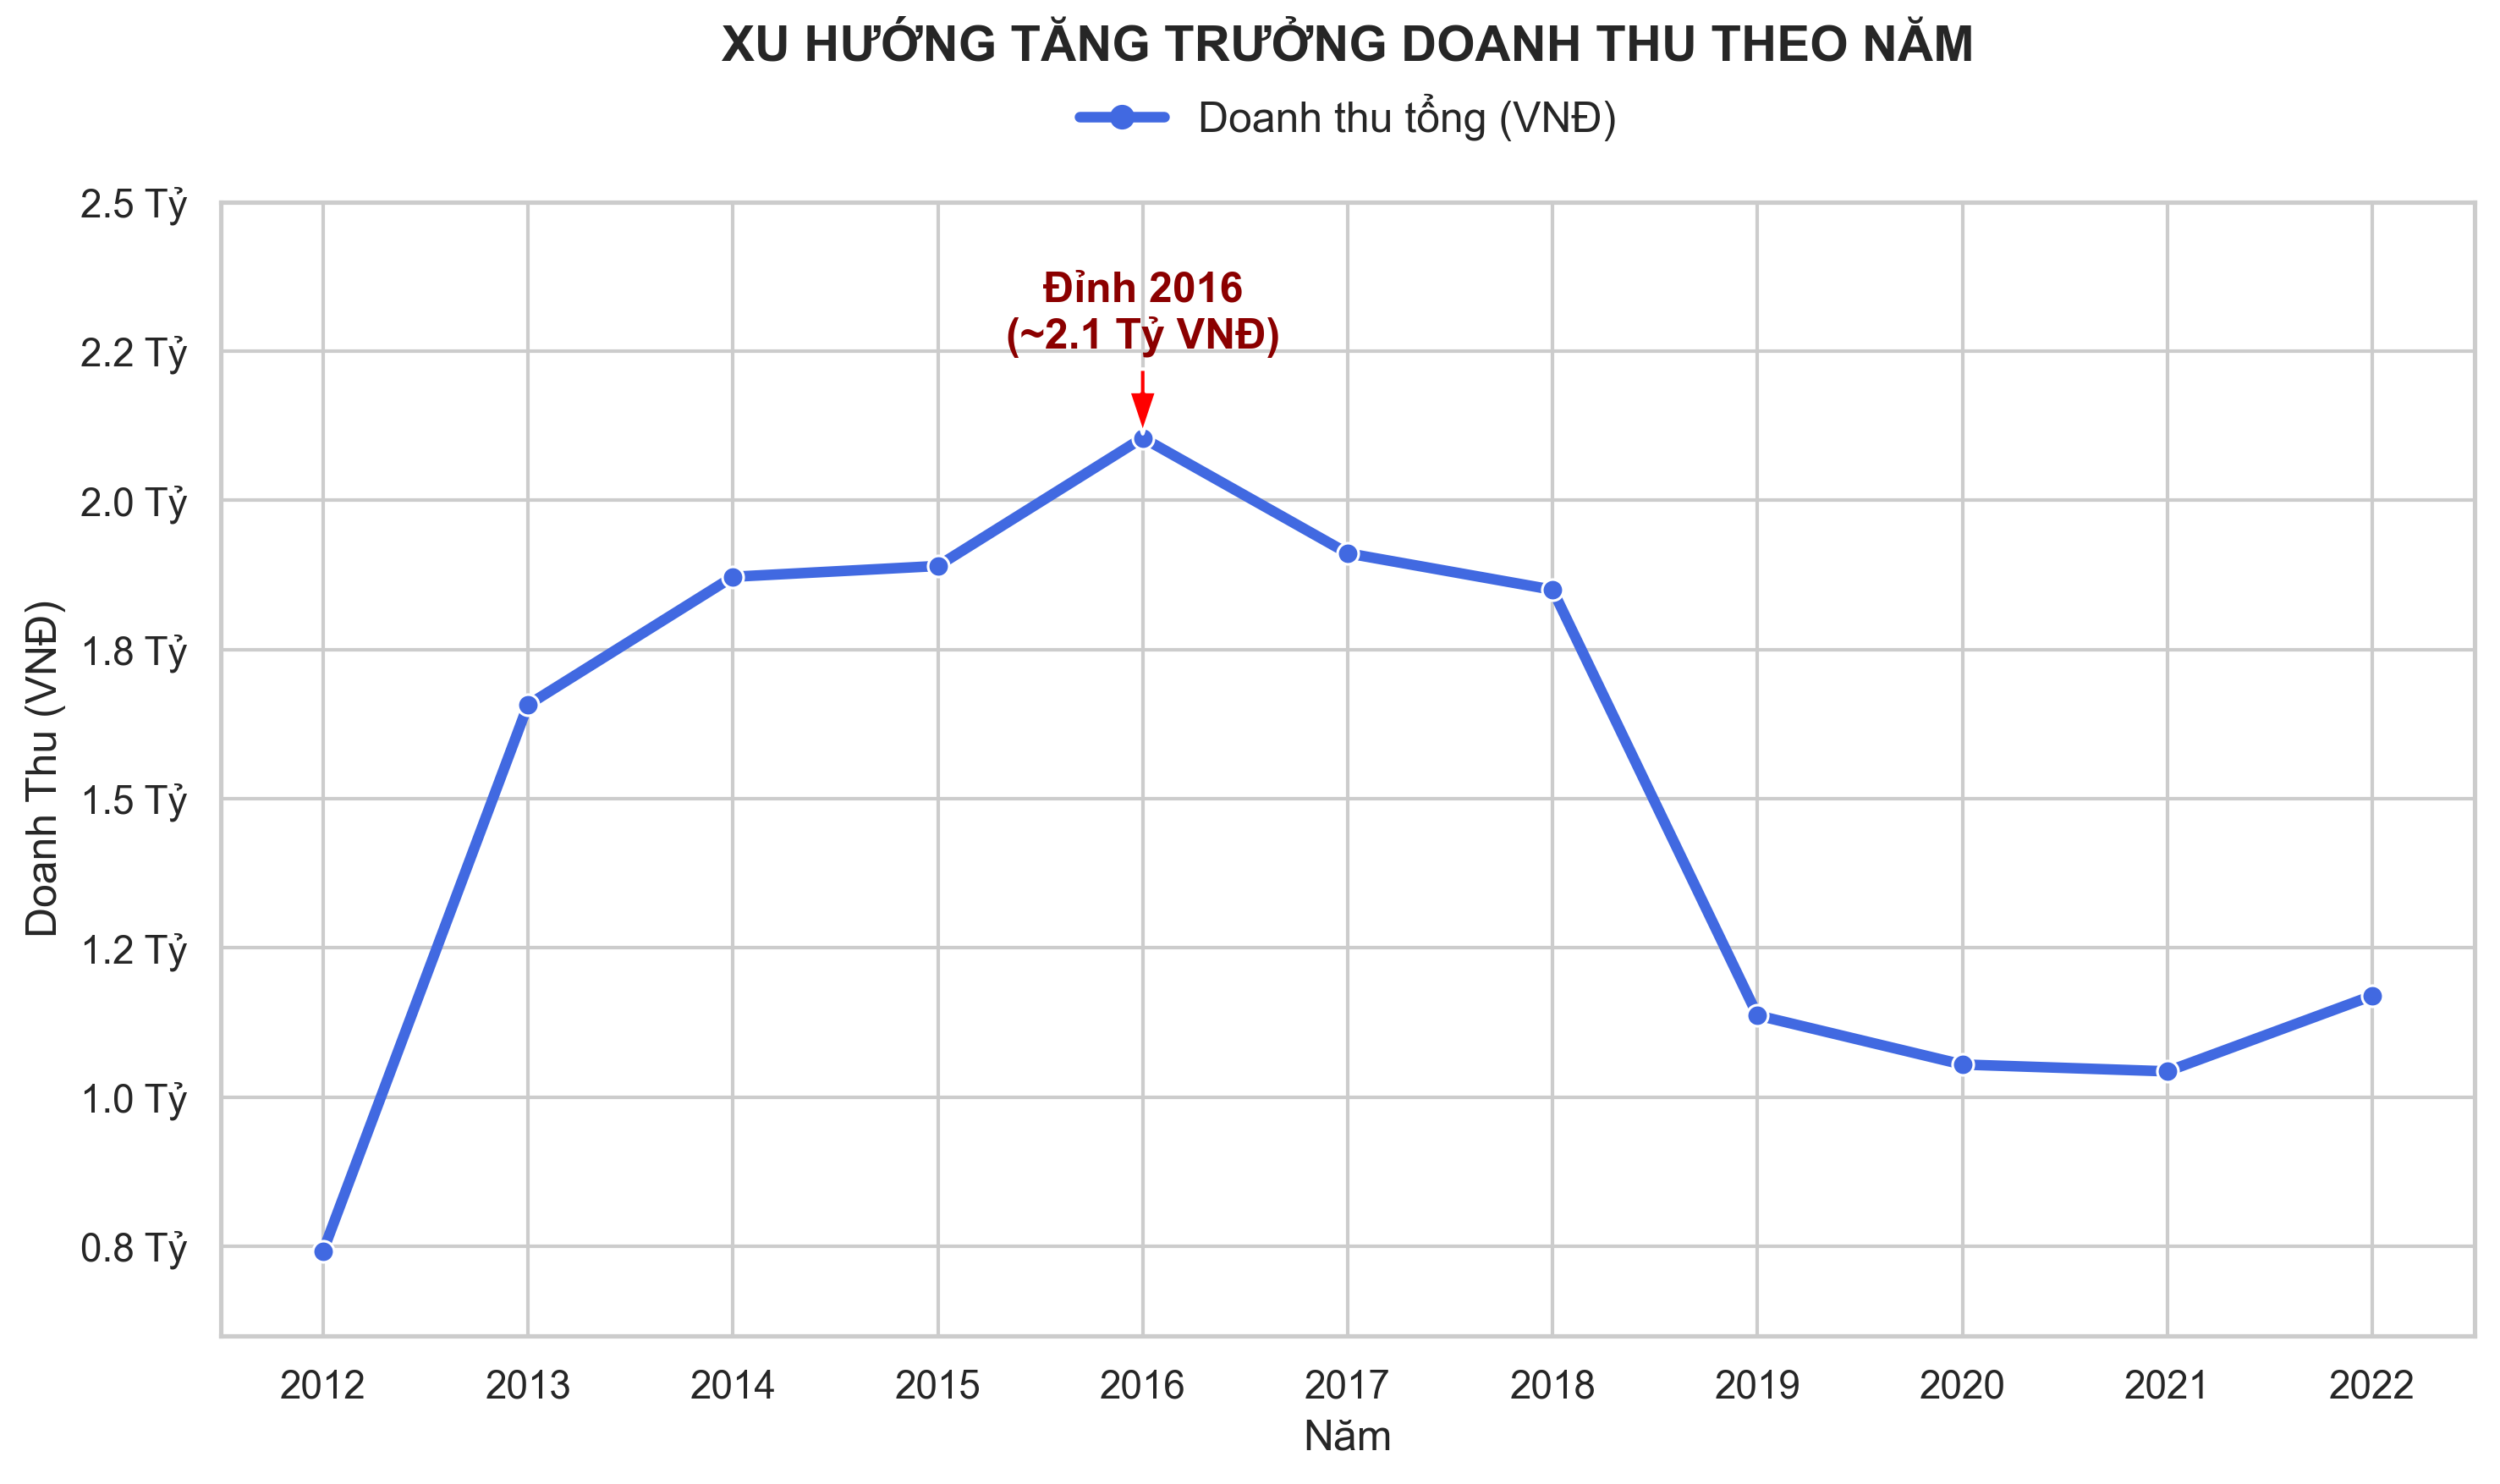
\includegraphics[width=0.48\textwidth]{Images/4a_Revenue_Yearly.png}
    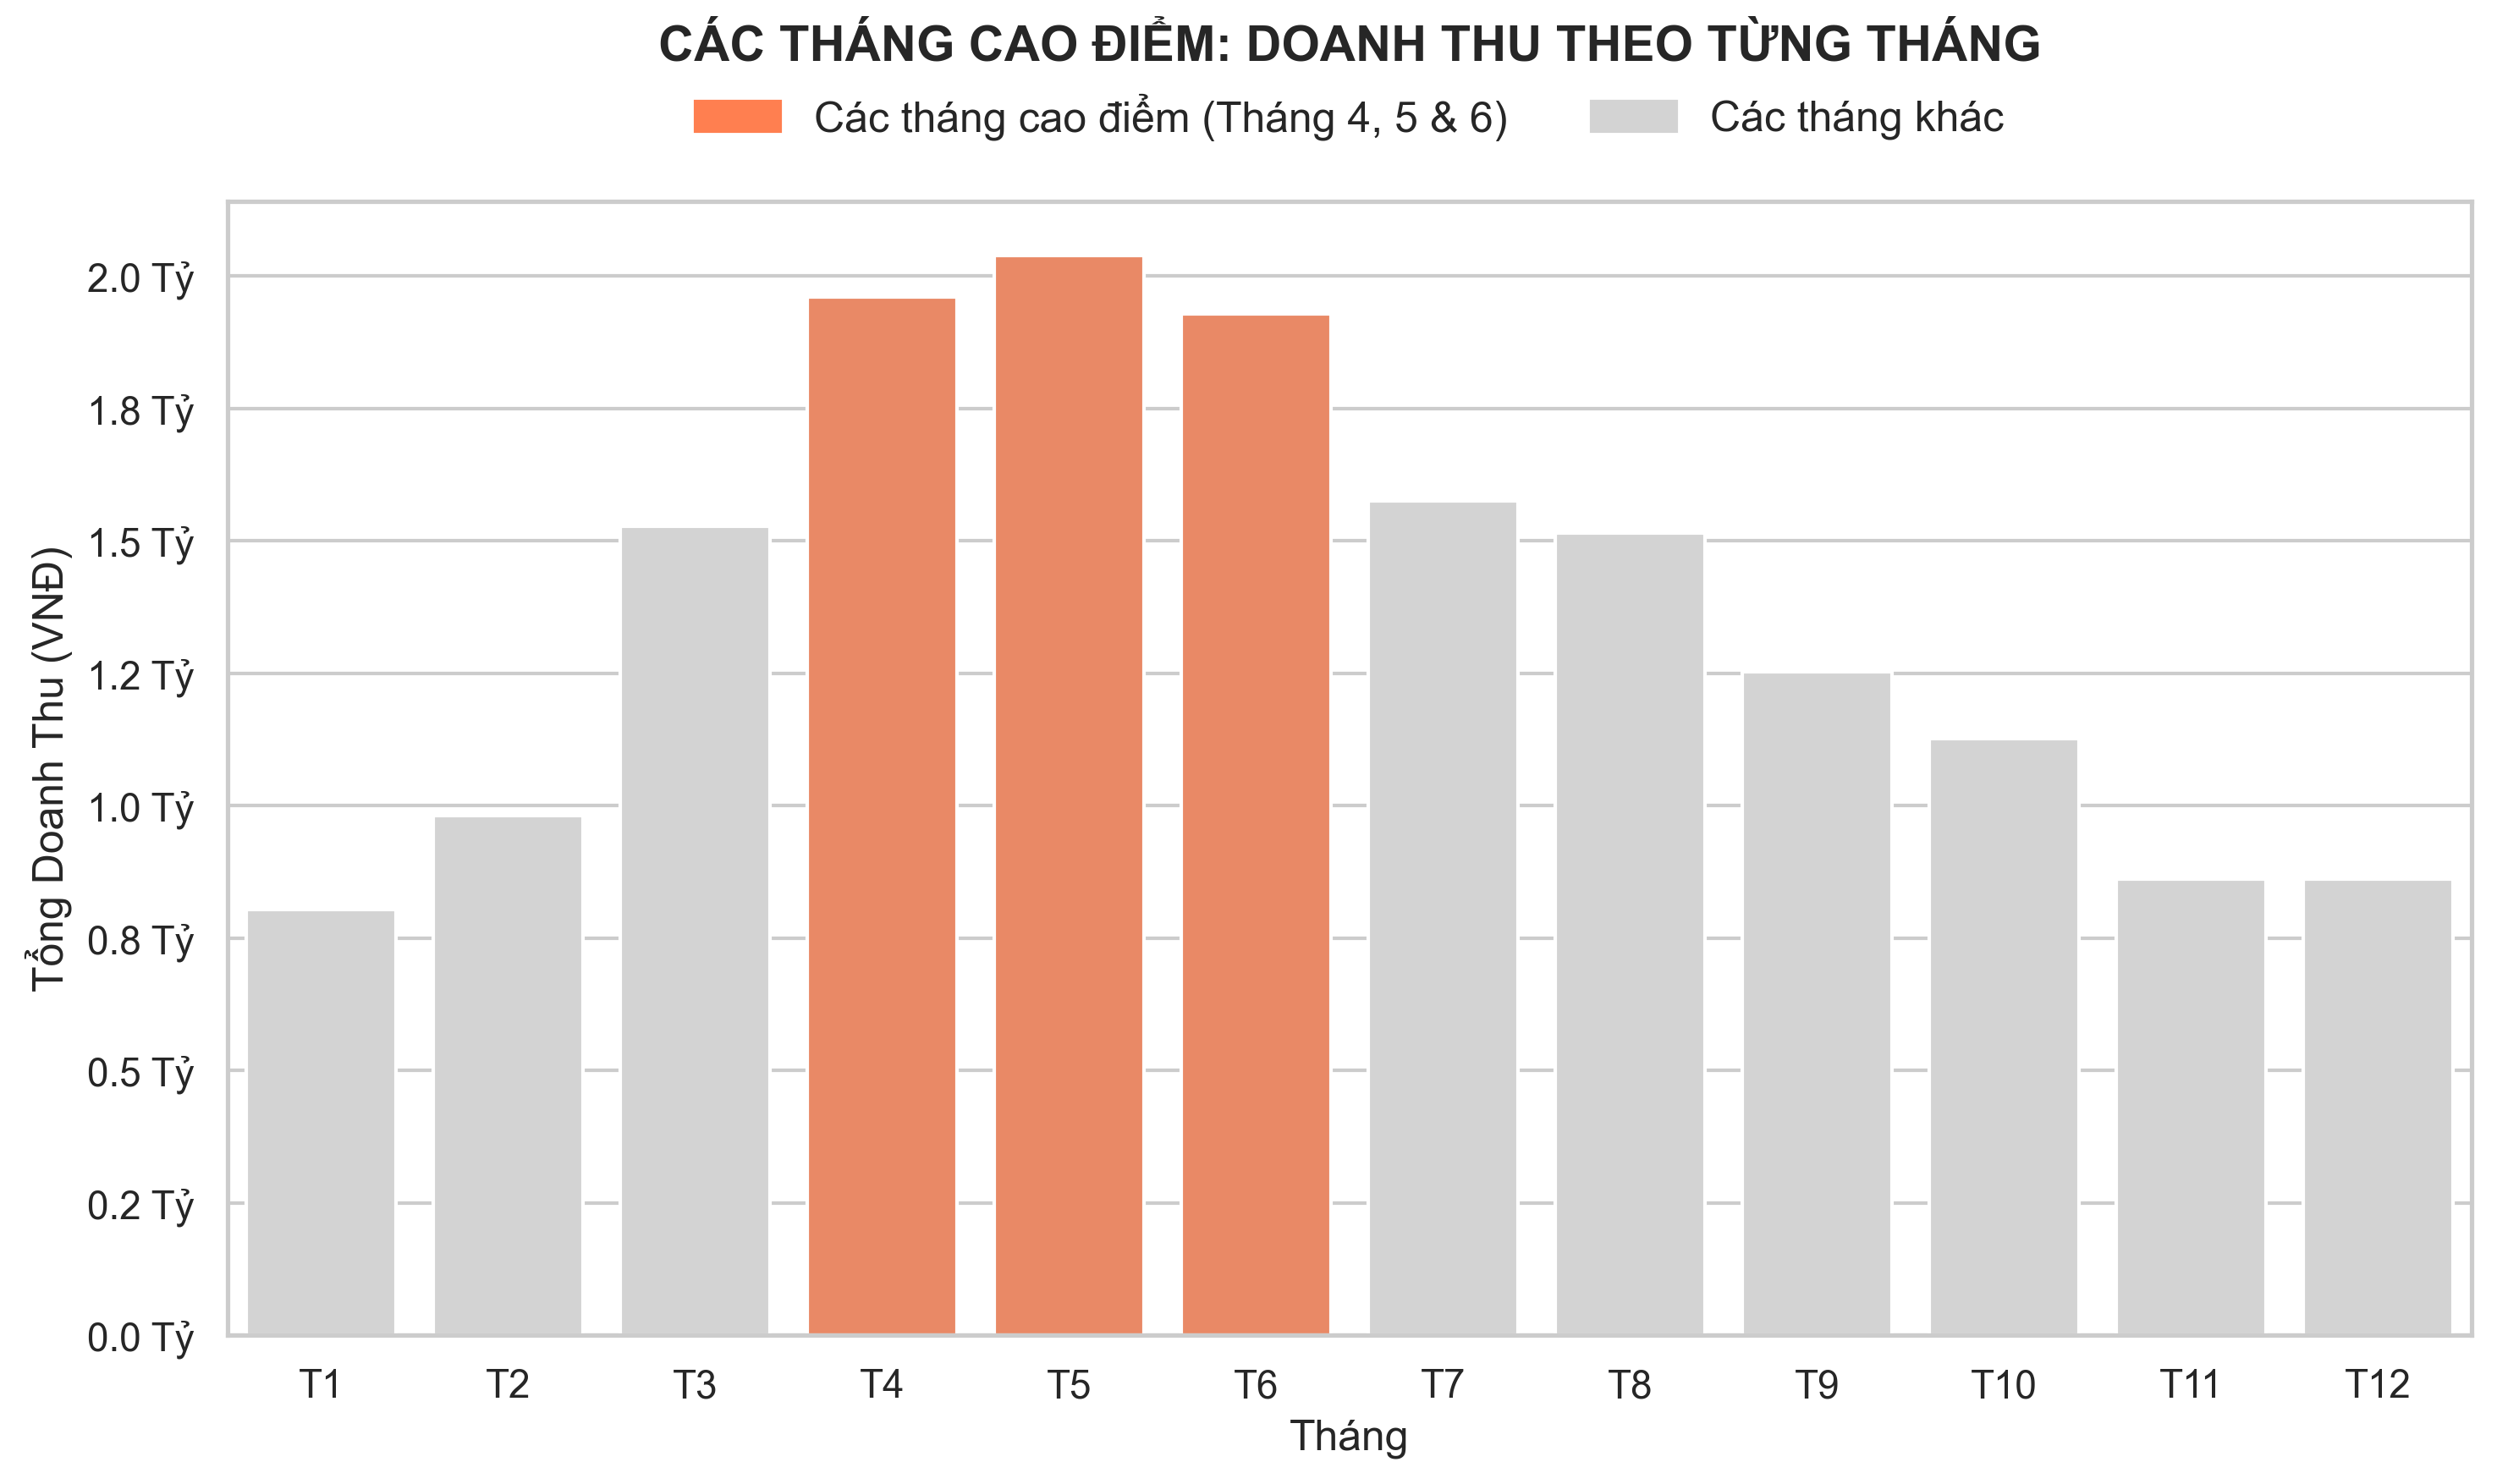
\includegraphics[width=0.48\textwidth]{Images/4b_Revenue_Monthly.png}
    \caption{(Trái) Xu hướng doanh thu 2013--2022, 3 giai đoạn rõ rệt. (Phải) Đỉnh doanh thu Quý 2.}
    \label{fig:revenue}
\end{figure}

\subsection*{Khủng Hoảng Biên Lợi Nhuận — ``The Profit Trap''}

Hai ``hố đen'' lợi nhuận được phát hiện qua phân tích Gross Margin:

\begin{itemize}
    \setlength{\itemsep}{1pt}
    \item \textbf{Tháng 8 năm lẻ:} Voucher trợ giá cố định (50 VNĐ) gây bùng nổ chi phí gấp 10$\times$, đẩy Gross Margin xuống $-35\%$.
    \item \textbf{Tháng 12:} Chiến dịch ``sale chồng sale'' nén biên lợi nhuận xuống $1\text{--}2\%$ dù doanh thu bùng nổ.
\end{itemize}

\begin{figure}[H]
    \centering
    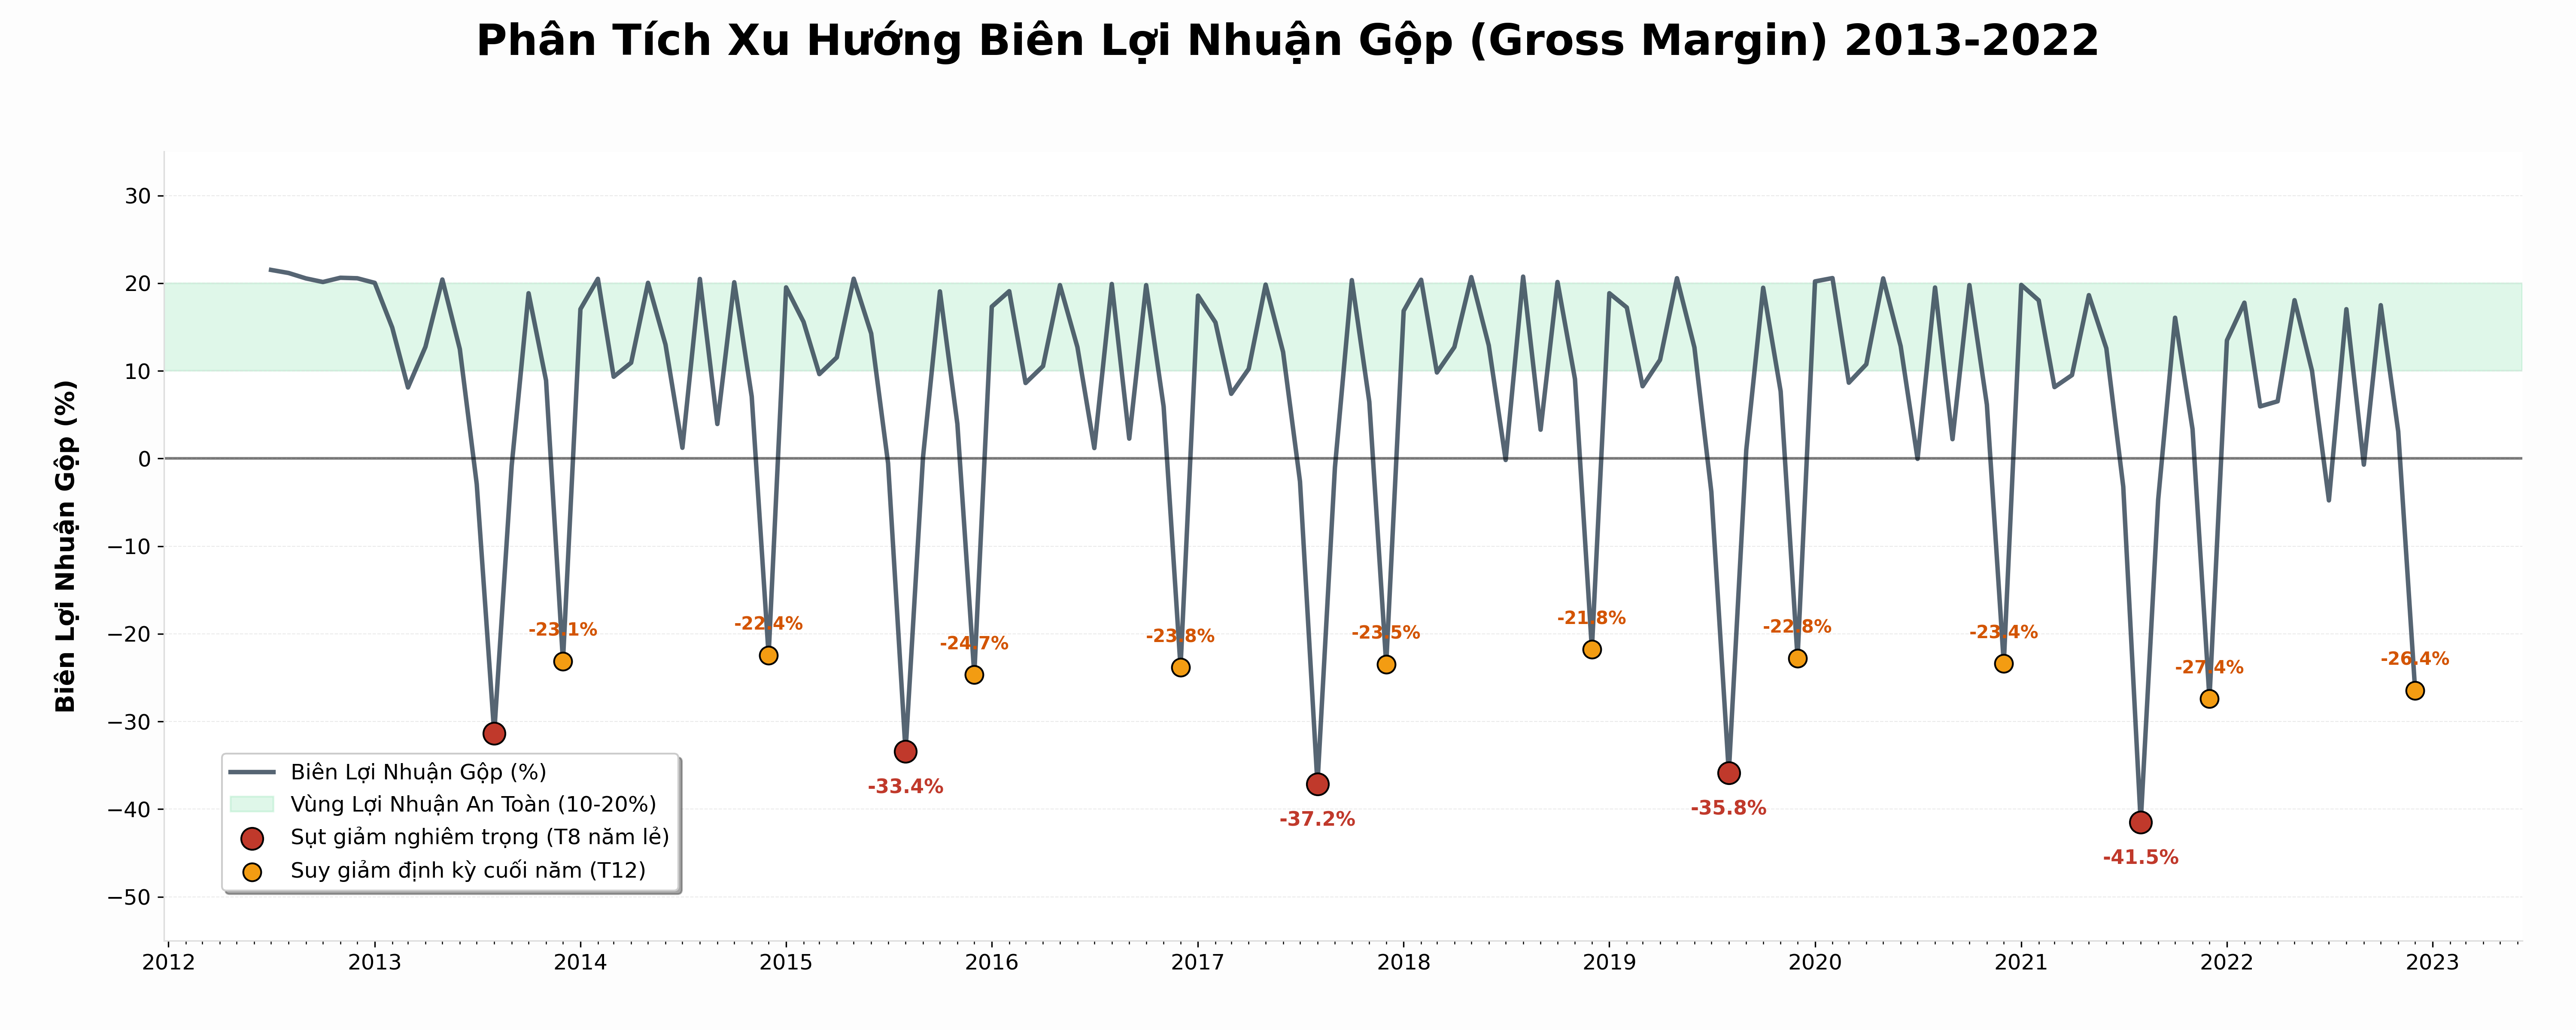
\includegraphics[width=0.48\textwidth]{Images/6a_Gross_Margin_Trend.png}
    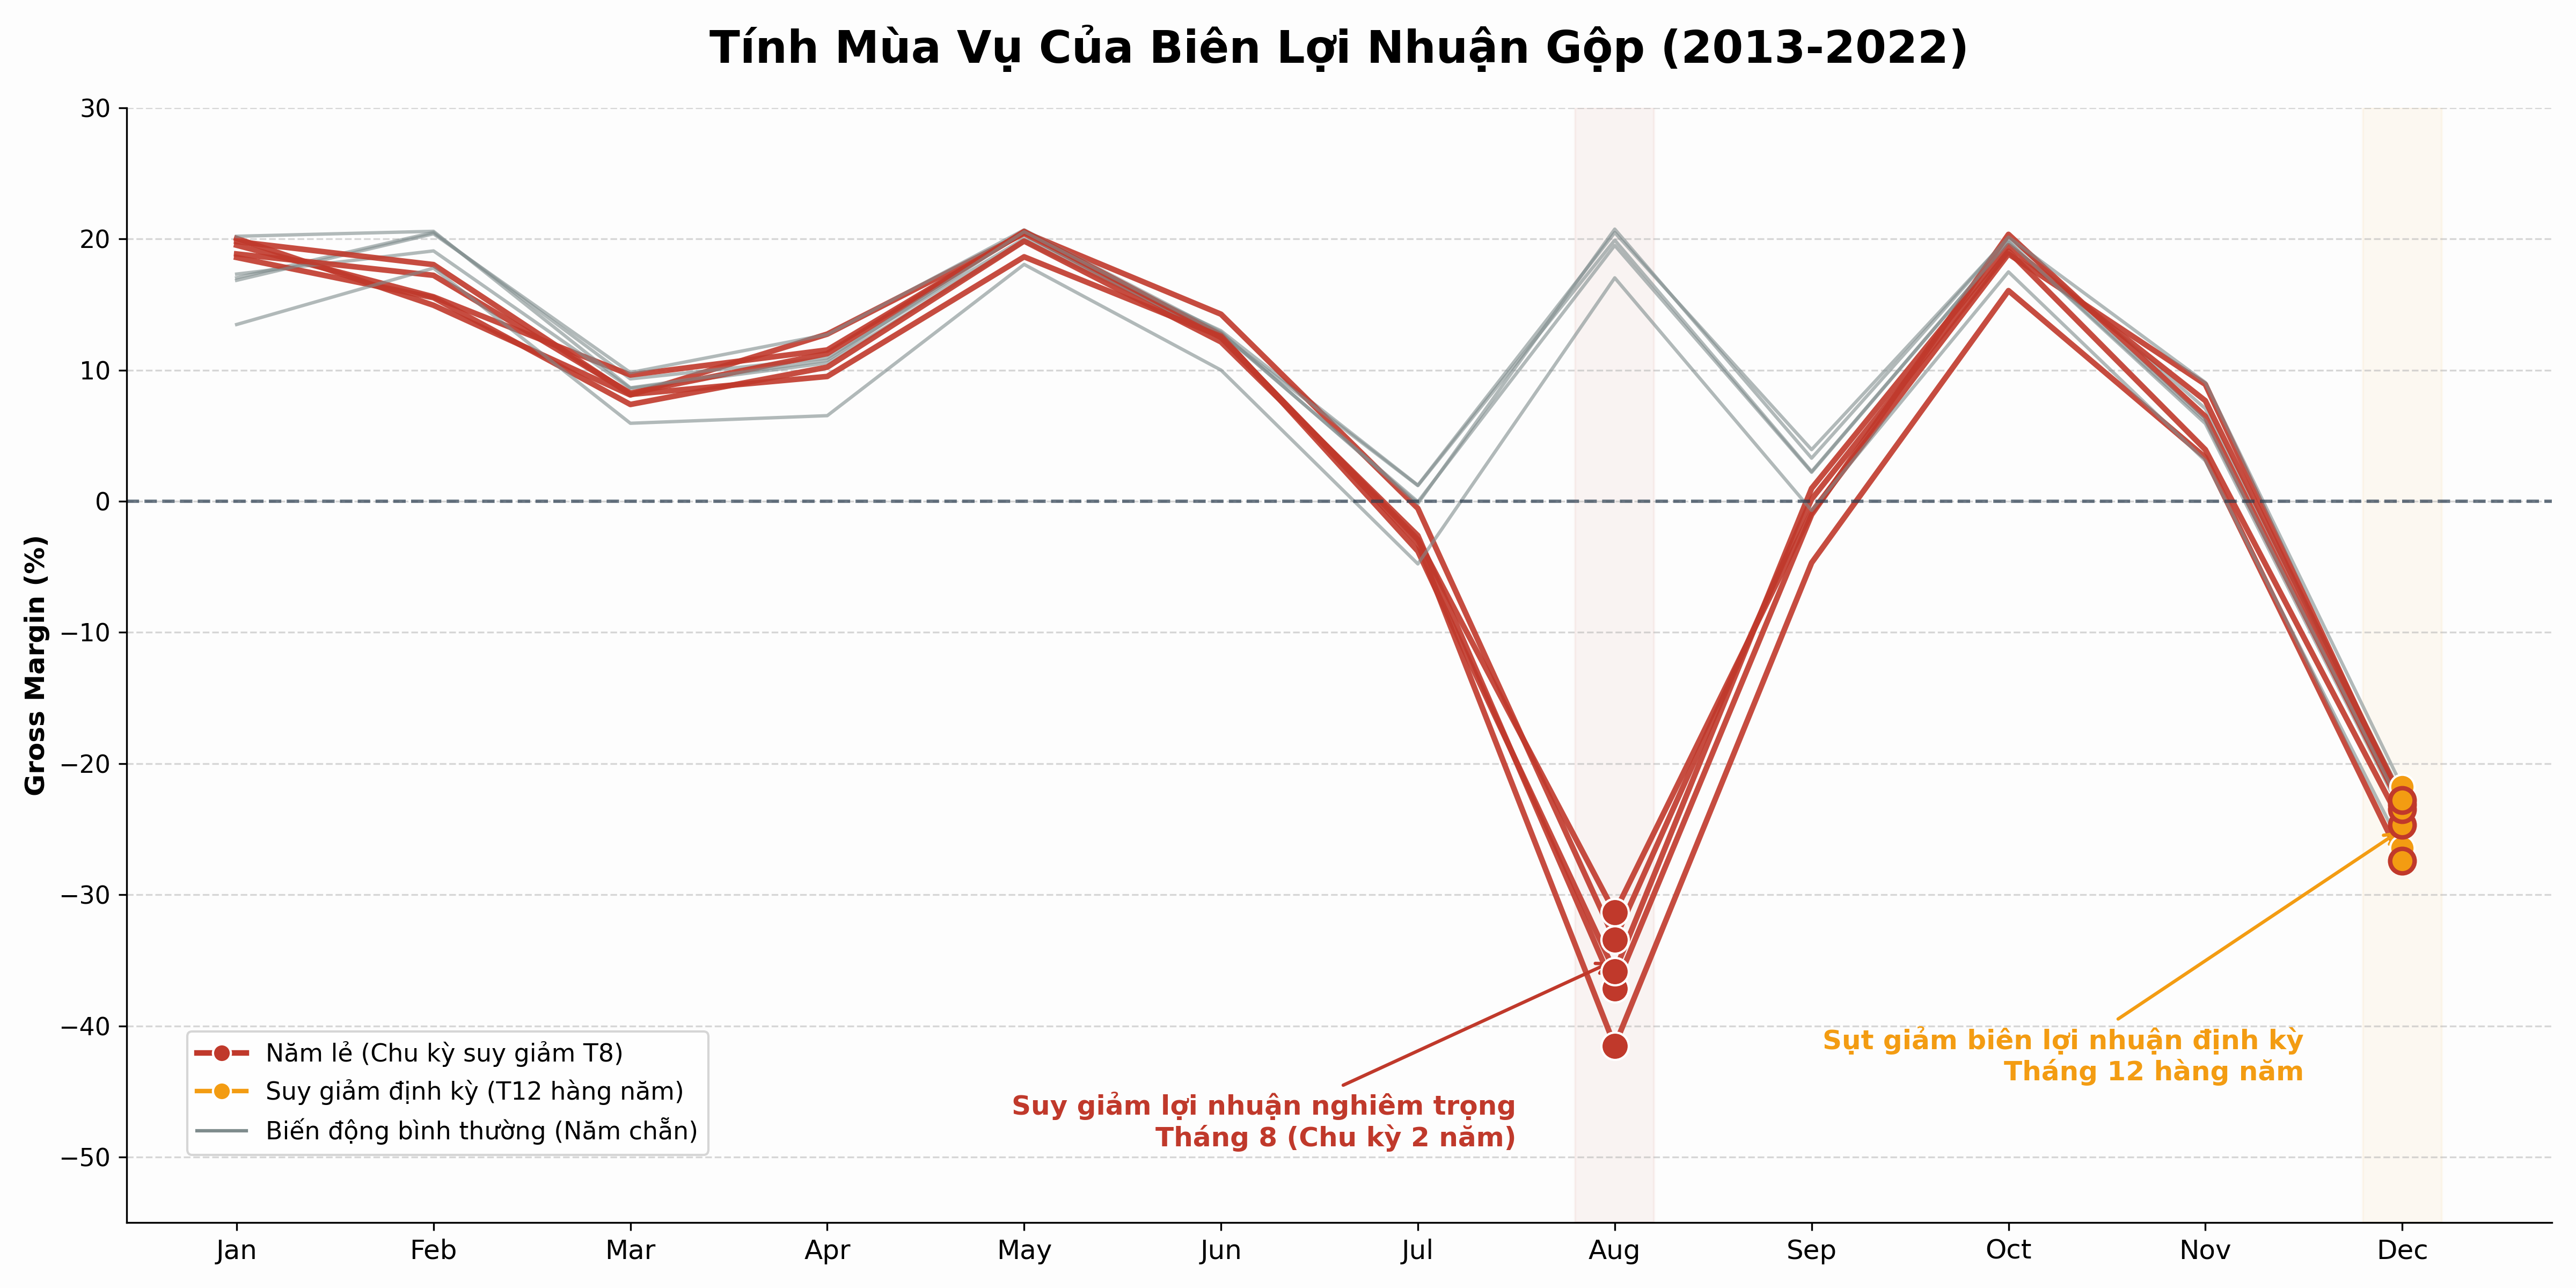
\includegraphics[width=0.48\textwidth]{Images/6b_Gross_Margin_Seasonality.png}
    \caption{(Trái) Suy giảm biên lợi nhuận dài hạn. (Phải) Chu kỳ khủng hoảng mùa vụ — T8 \& T12.}
    \label{fig:margin}
\end{figure}

\subsection*{Nghịch Lý Khuyến Mãi \& Điểm Nghẽn Mobile}

\textbf{Promotion Paradox:} Đơn hàng áp mã giảm giá ($38.4\%$ tổng đơn) có AOV thấp hơn $20.5\%$ so với đơn nguyên giá (21.914 vs 27.565 VNĐ). Kiểm toán 6 chiến dịch cho thấy 5/6 chiến dịch lỗ ròng, đỉnh điểm Urban Blowout: $-62.5\%$ biên lợi nhuận.

\textbf{Mobile Friction:} Kênh di động dẫn đầu lưu lượng ($45.1\%$) nhưng tỷ lệ bỏ giỏ hàng lên tới $68.5\%$. Thời lượng lưu trang trung bình 160s chứng minh ý định mua sắm rõ ràng — điểm nghẽn UX tại bước thanh toán.

\begin{figure}[H]
    \centering
    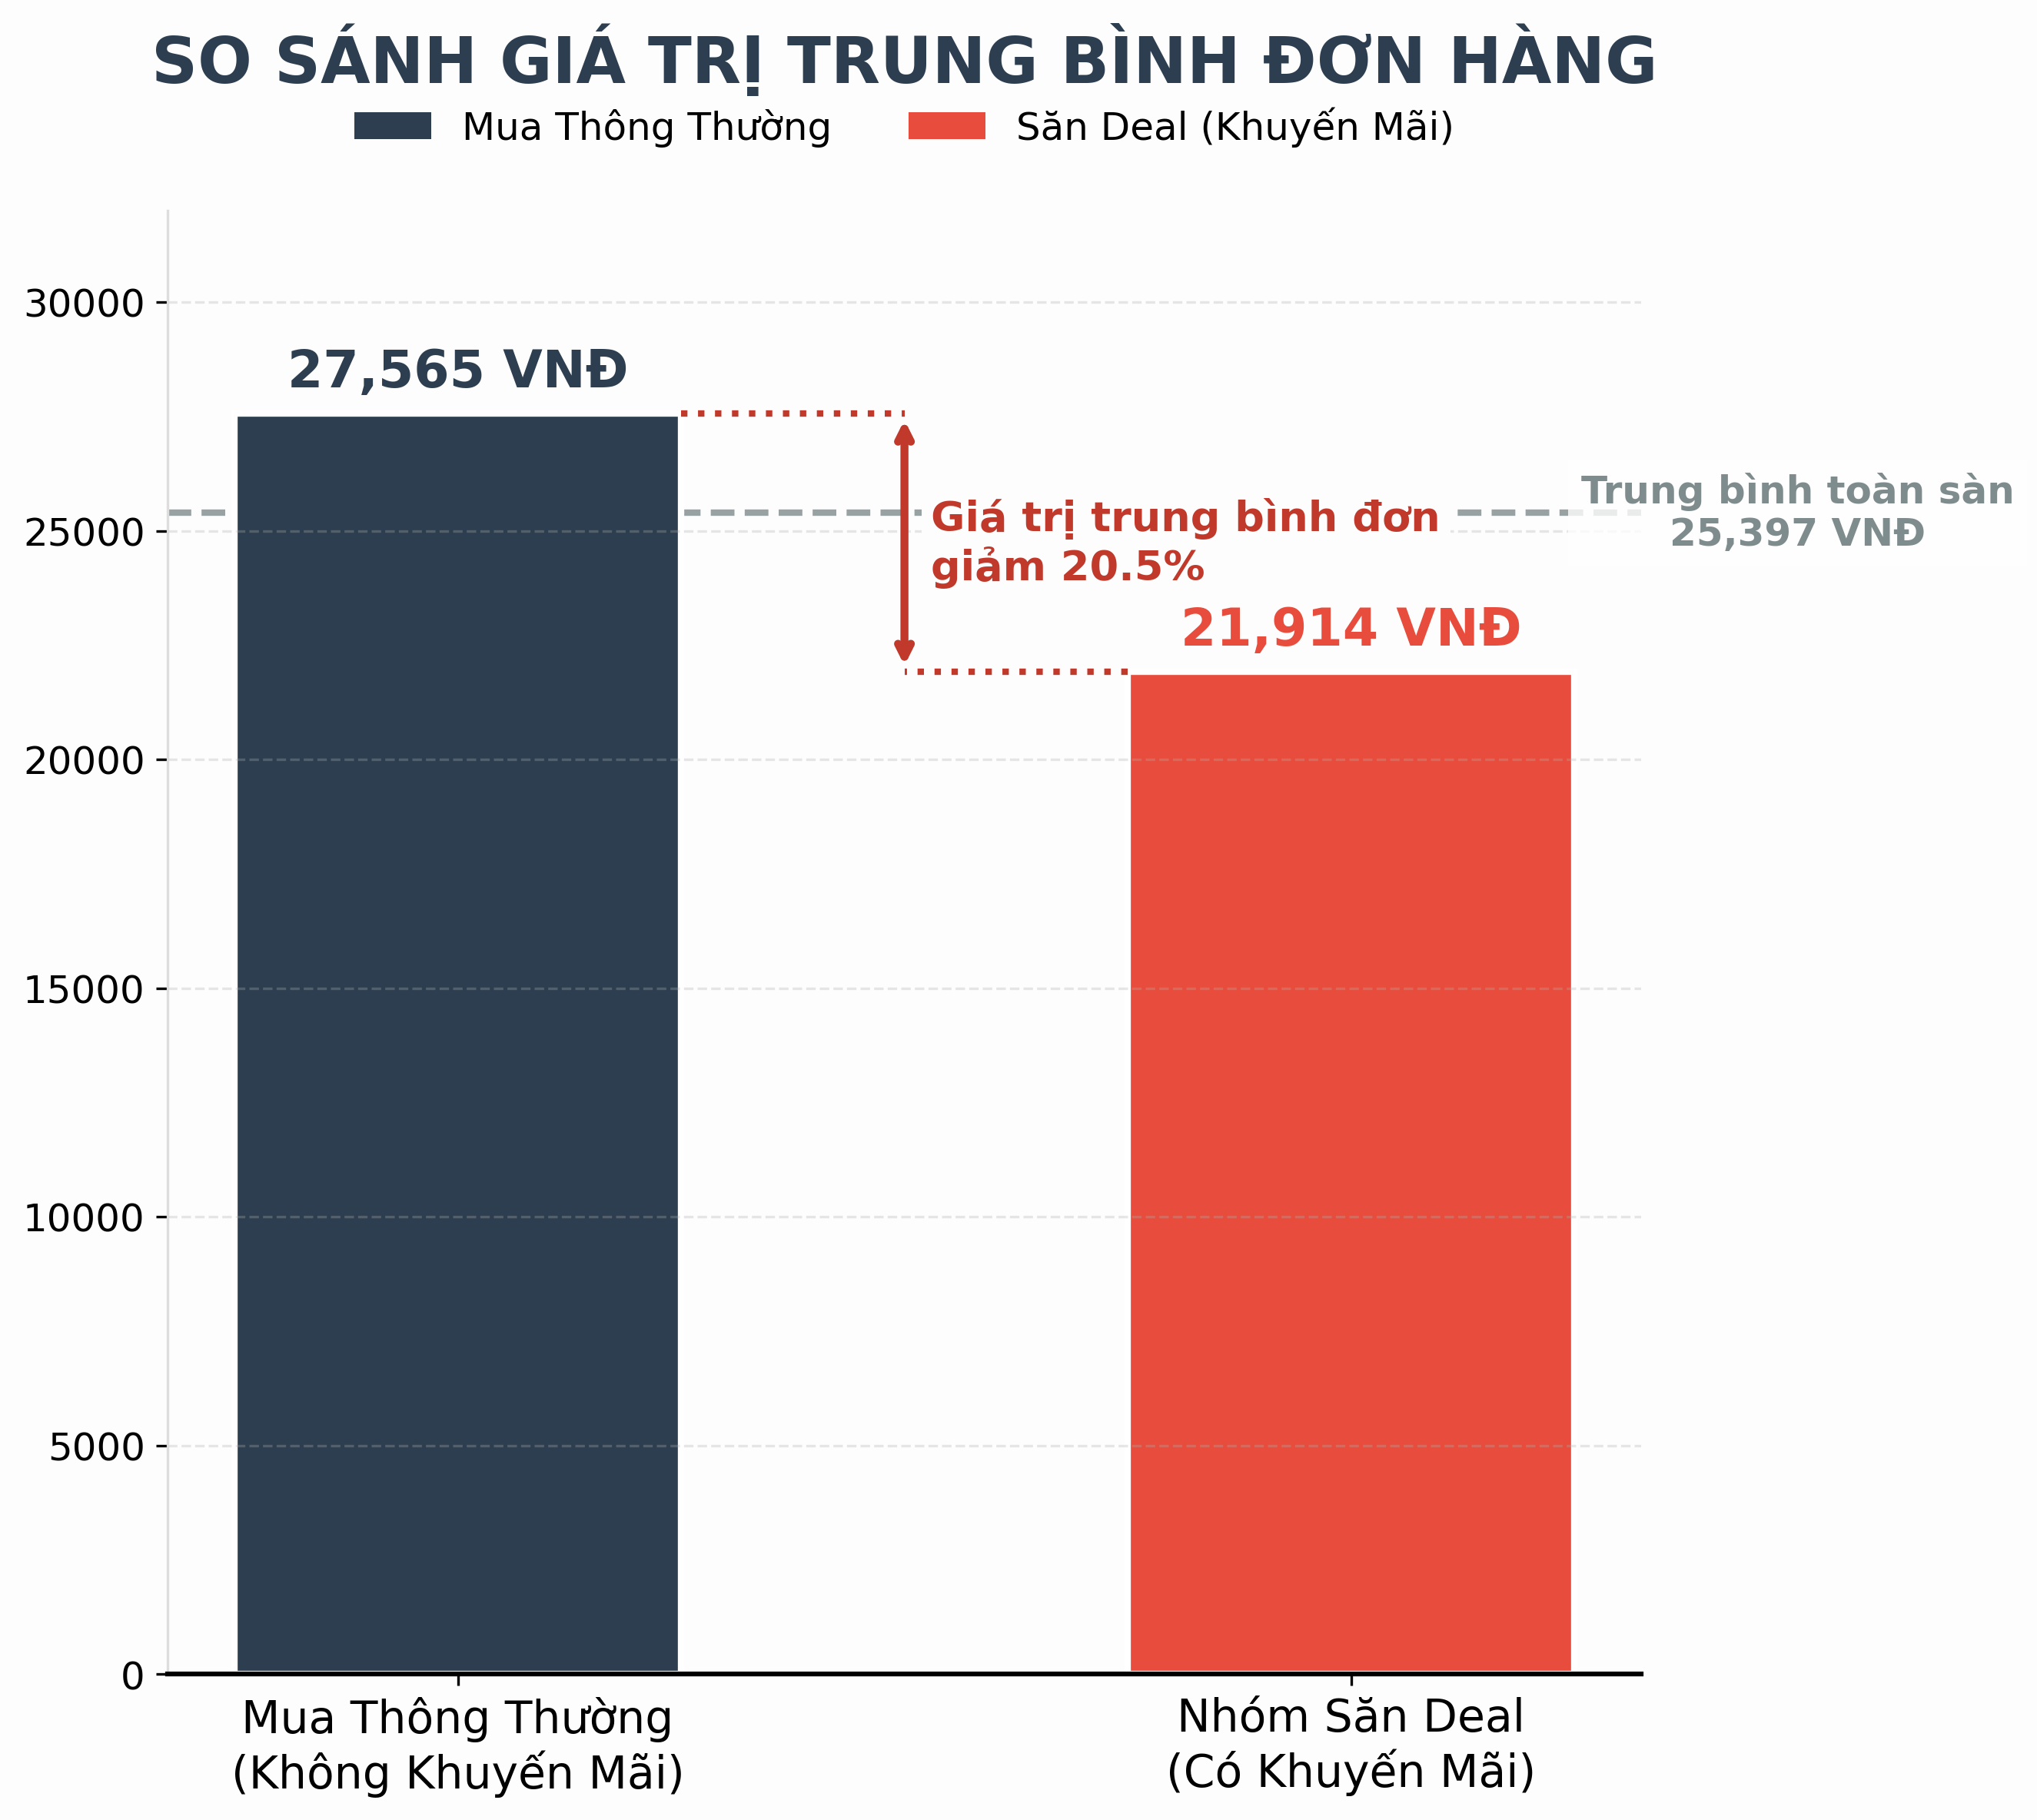
\includegraphics[width=0.48\textwidth]{Images/7b_Promotion_AOV.png}
    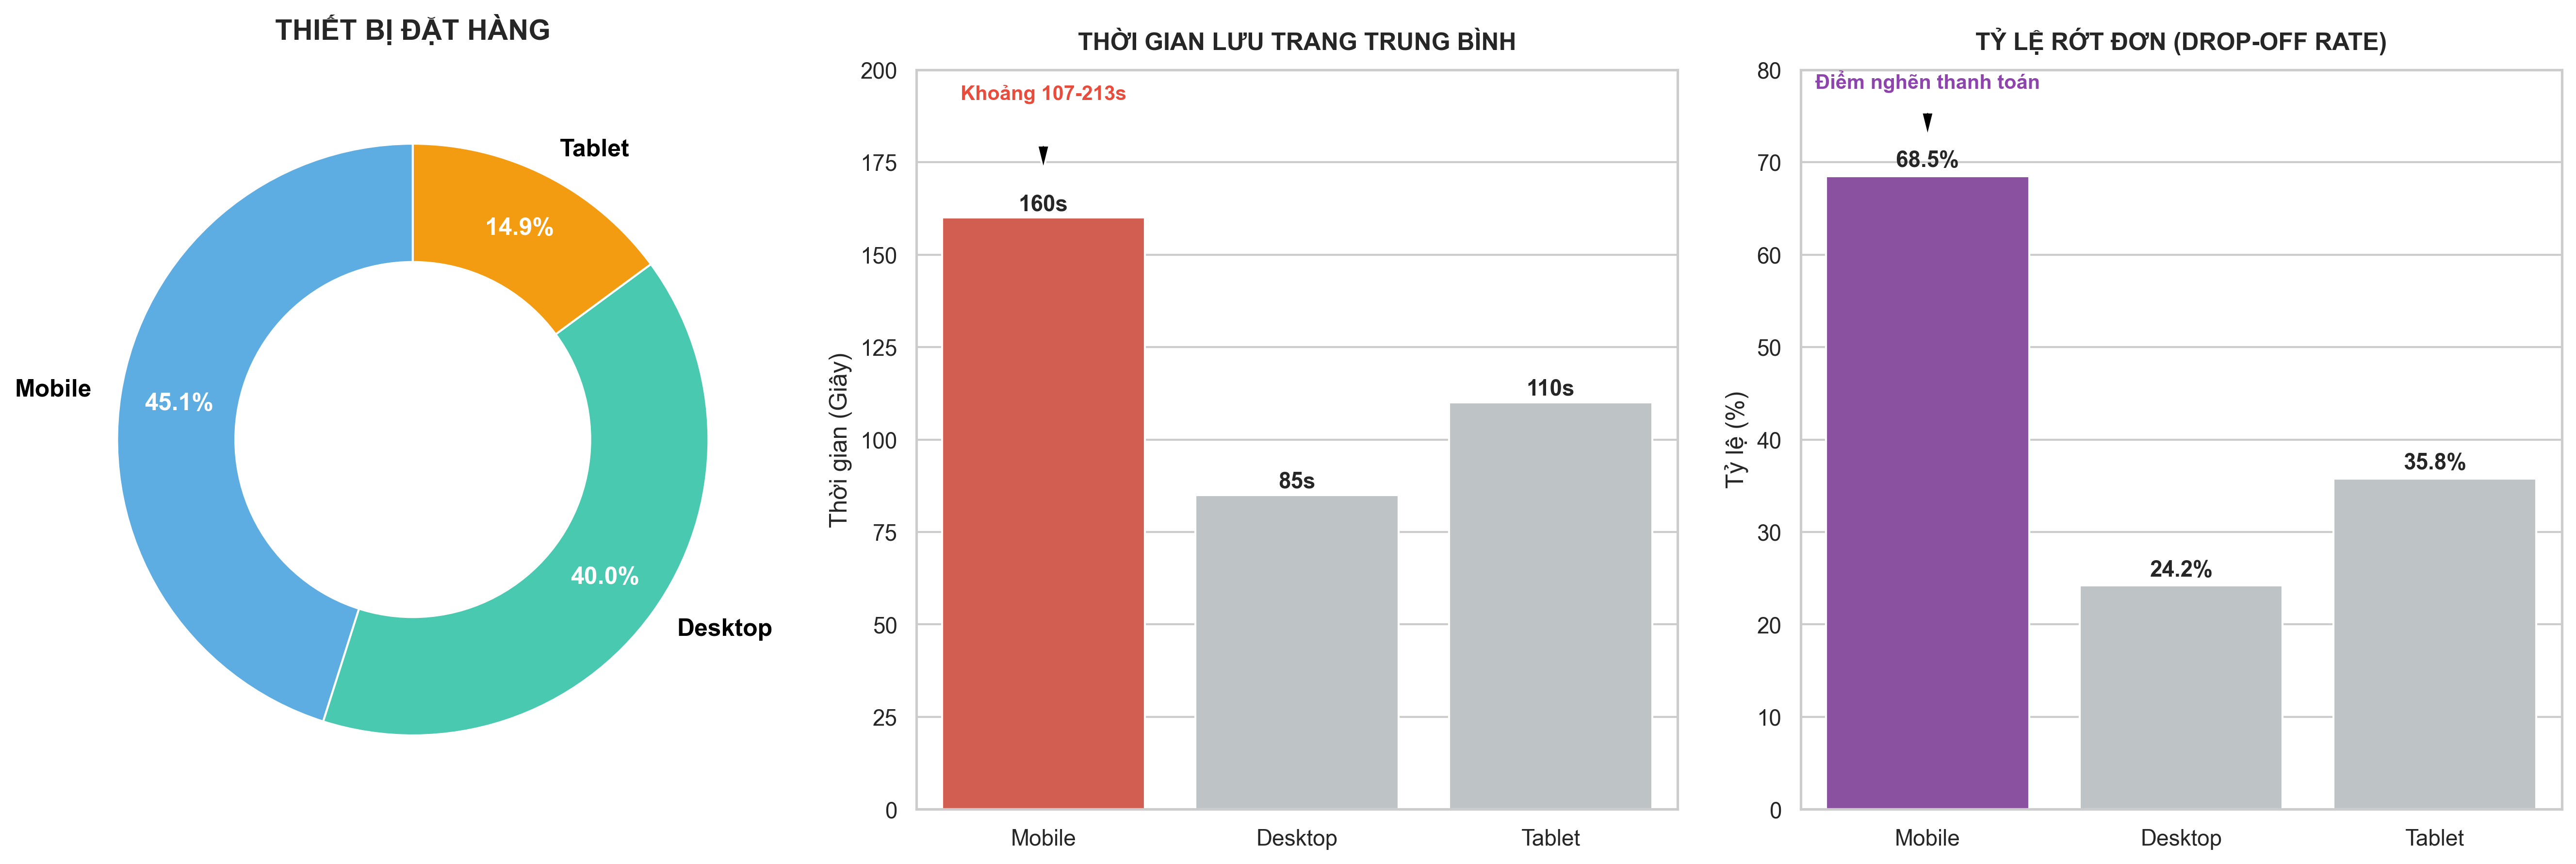
\includegraphics[width=0.48\textwidth]{Images/5a_Device_Composite.png}
    \caption{(Trái) AOV sụt giảm khi có khuyến mãi. (Phải) Mobile: traffic cao nhất, rớt đơn nhiều nhất.}
    \label{fig:promo_mobile}
\end{figure}

\subsection*{Chuỗi Cung Ứng \& Nghịch Lý Market-Fit}

Outdoor chiếm chỉ $9\%$ doanh thu nhưng Overstock Rate lên tới $80\%$, Sell-through Rate chạm đáy $14\%$. Network Graph Analysis nhận diện 3 SKU deadstock (MekongFit RS-10, HanoiStreet YY-04, UrbanVN RS-04) — paradox: rating 4--5 sao, return rate $\approx 0$, nhưng Degree Centrality cực thấp (0.02--0.05). Kết luận: \textit{Product-Market Mismatch}, không phải lỗi chất lượng.

\begin{figure}[H]
    \centering
    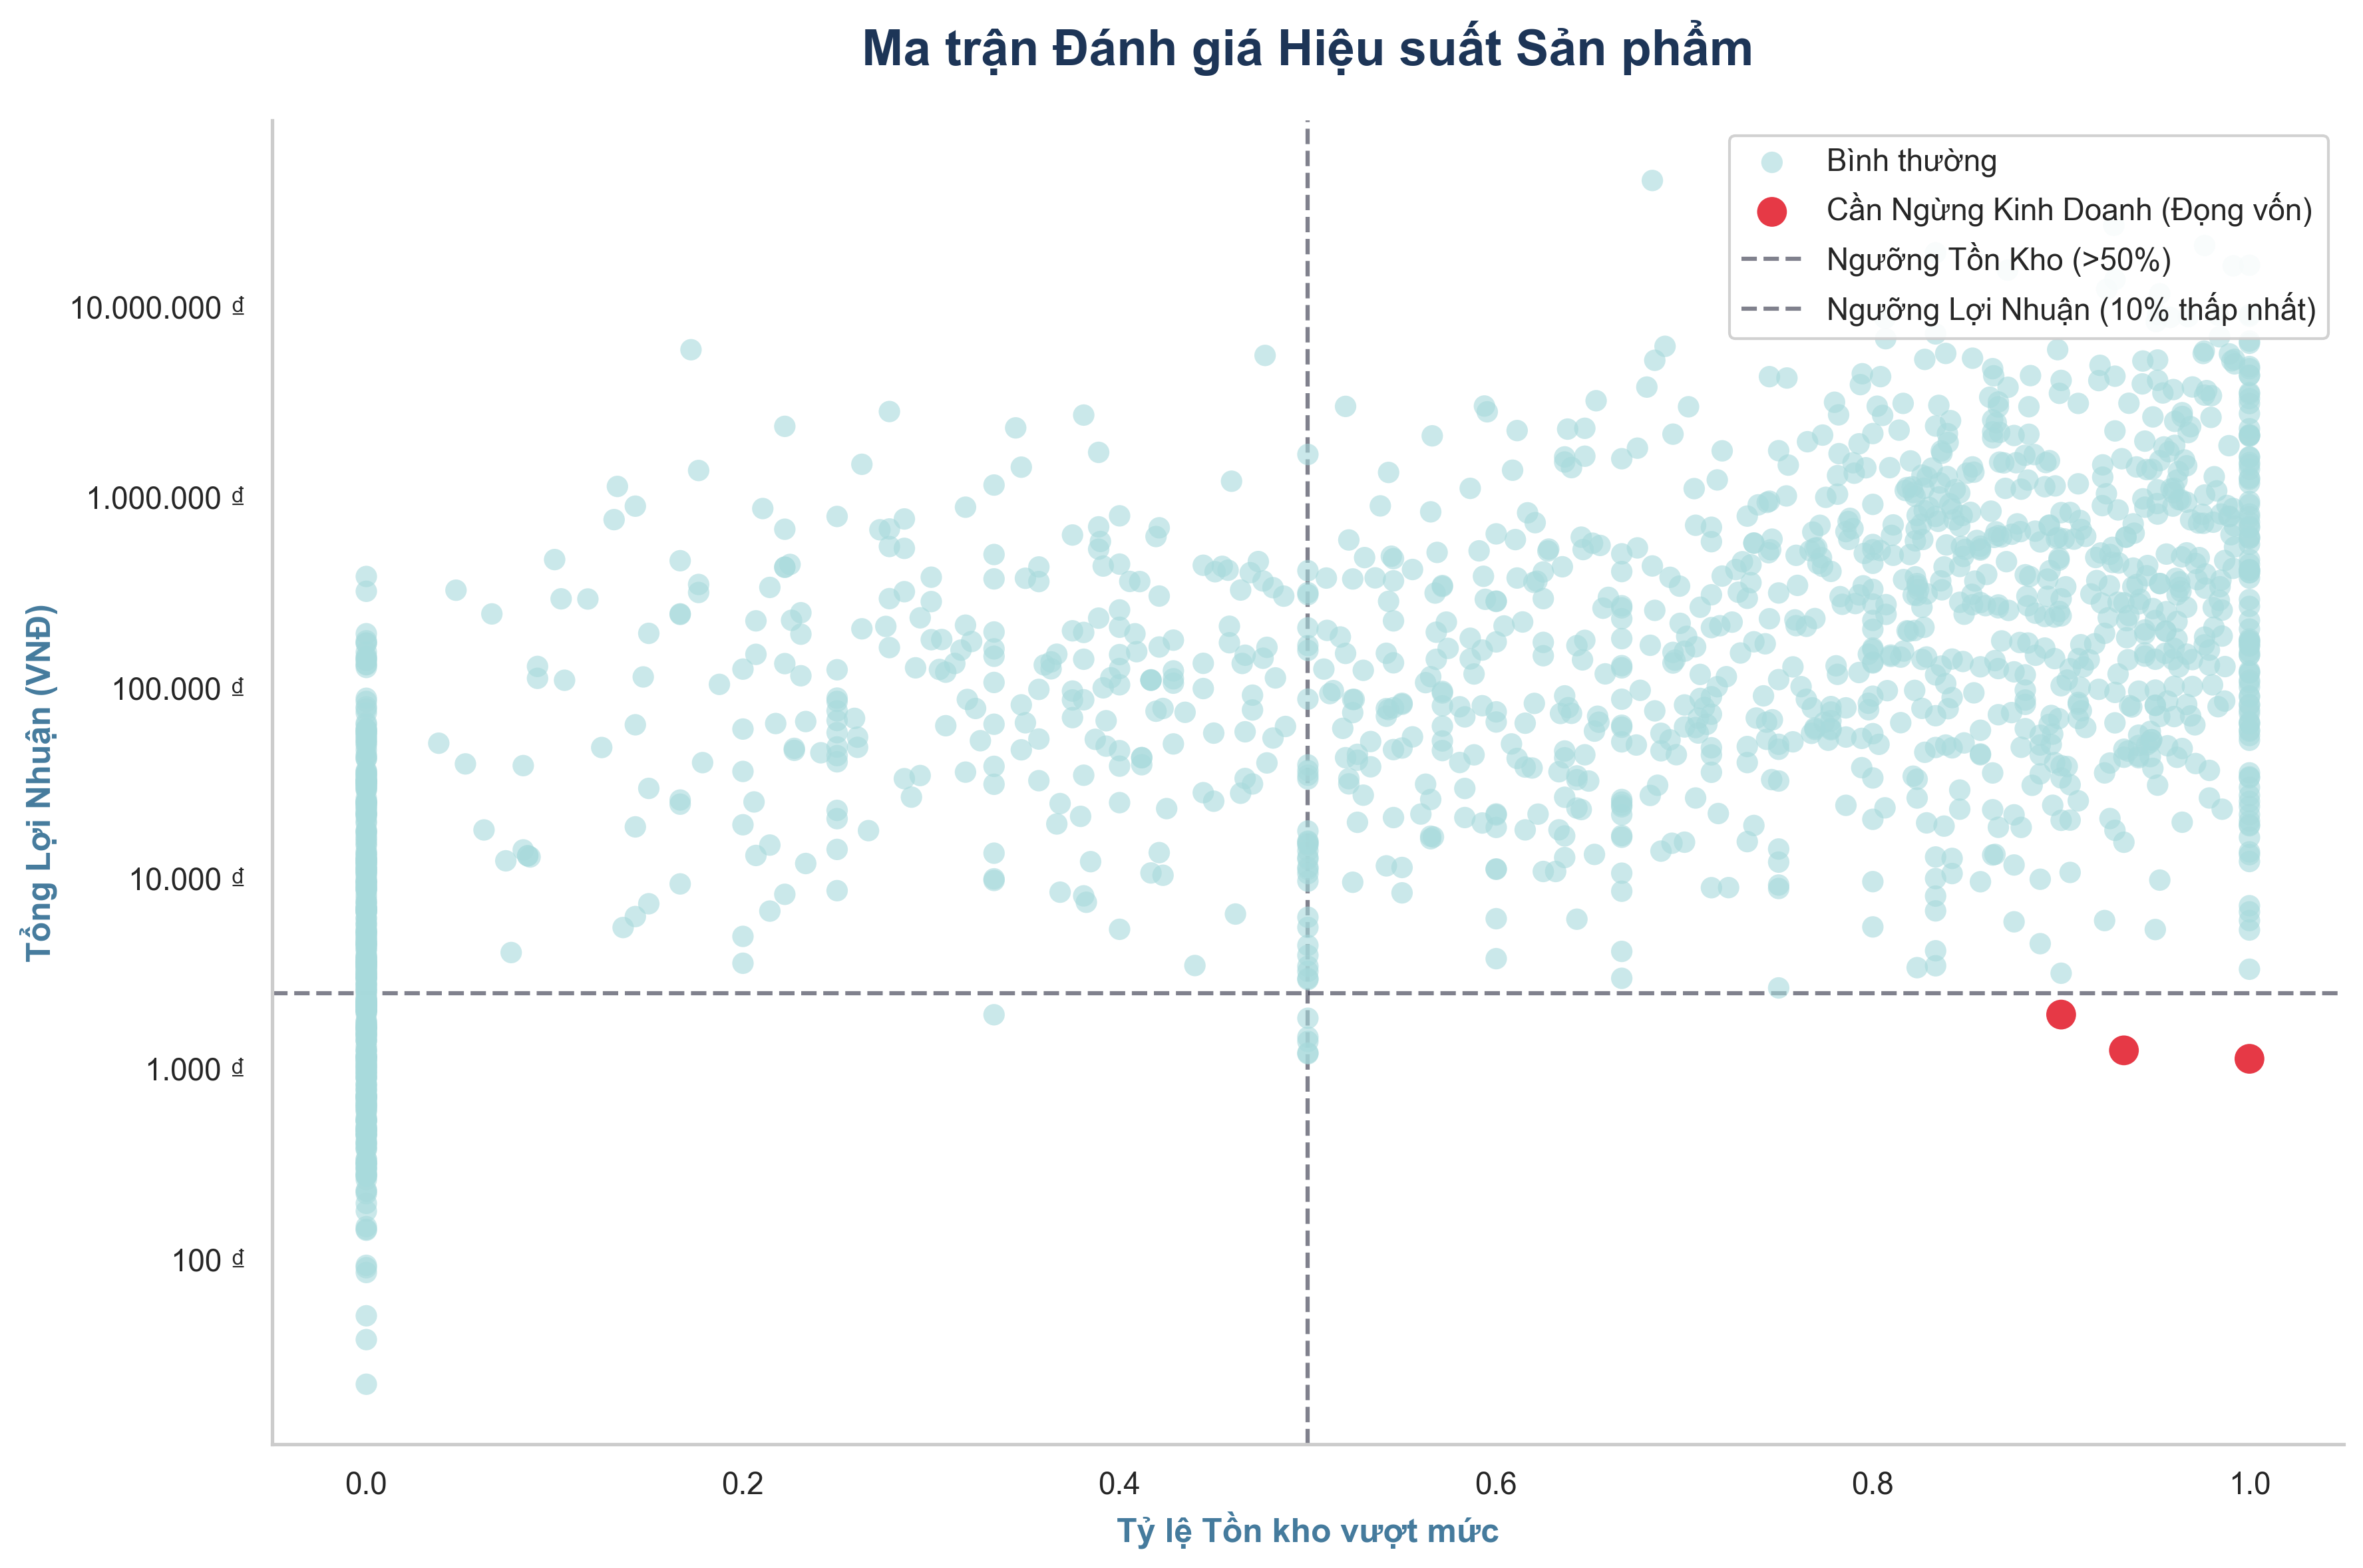
\includegraphics[width=0.48\textwidth]{Images/Story_1_Quadrant_Scatter.png}
    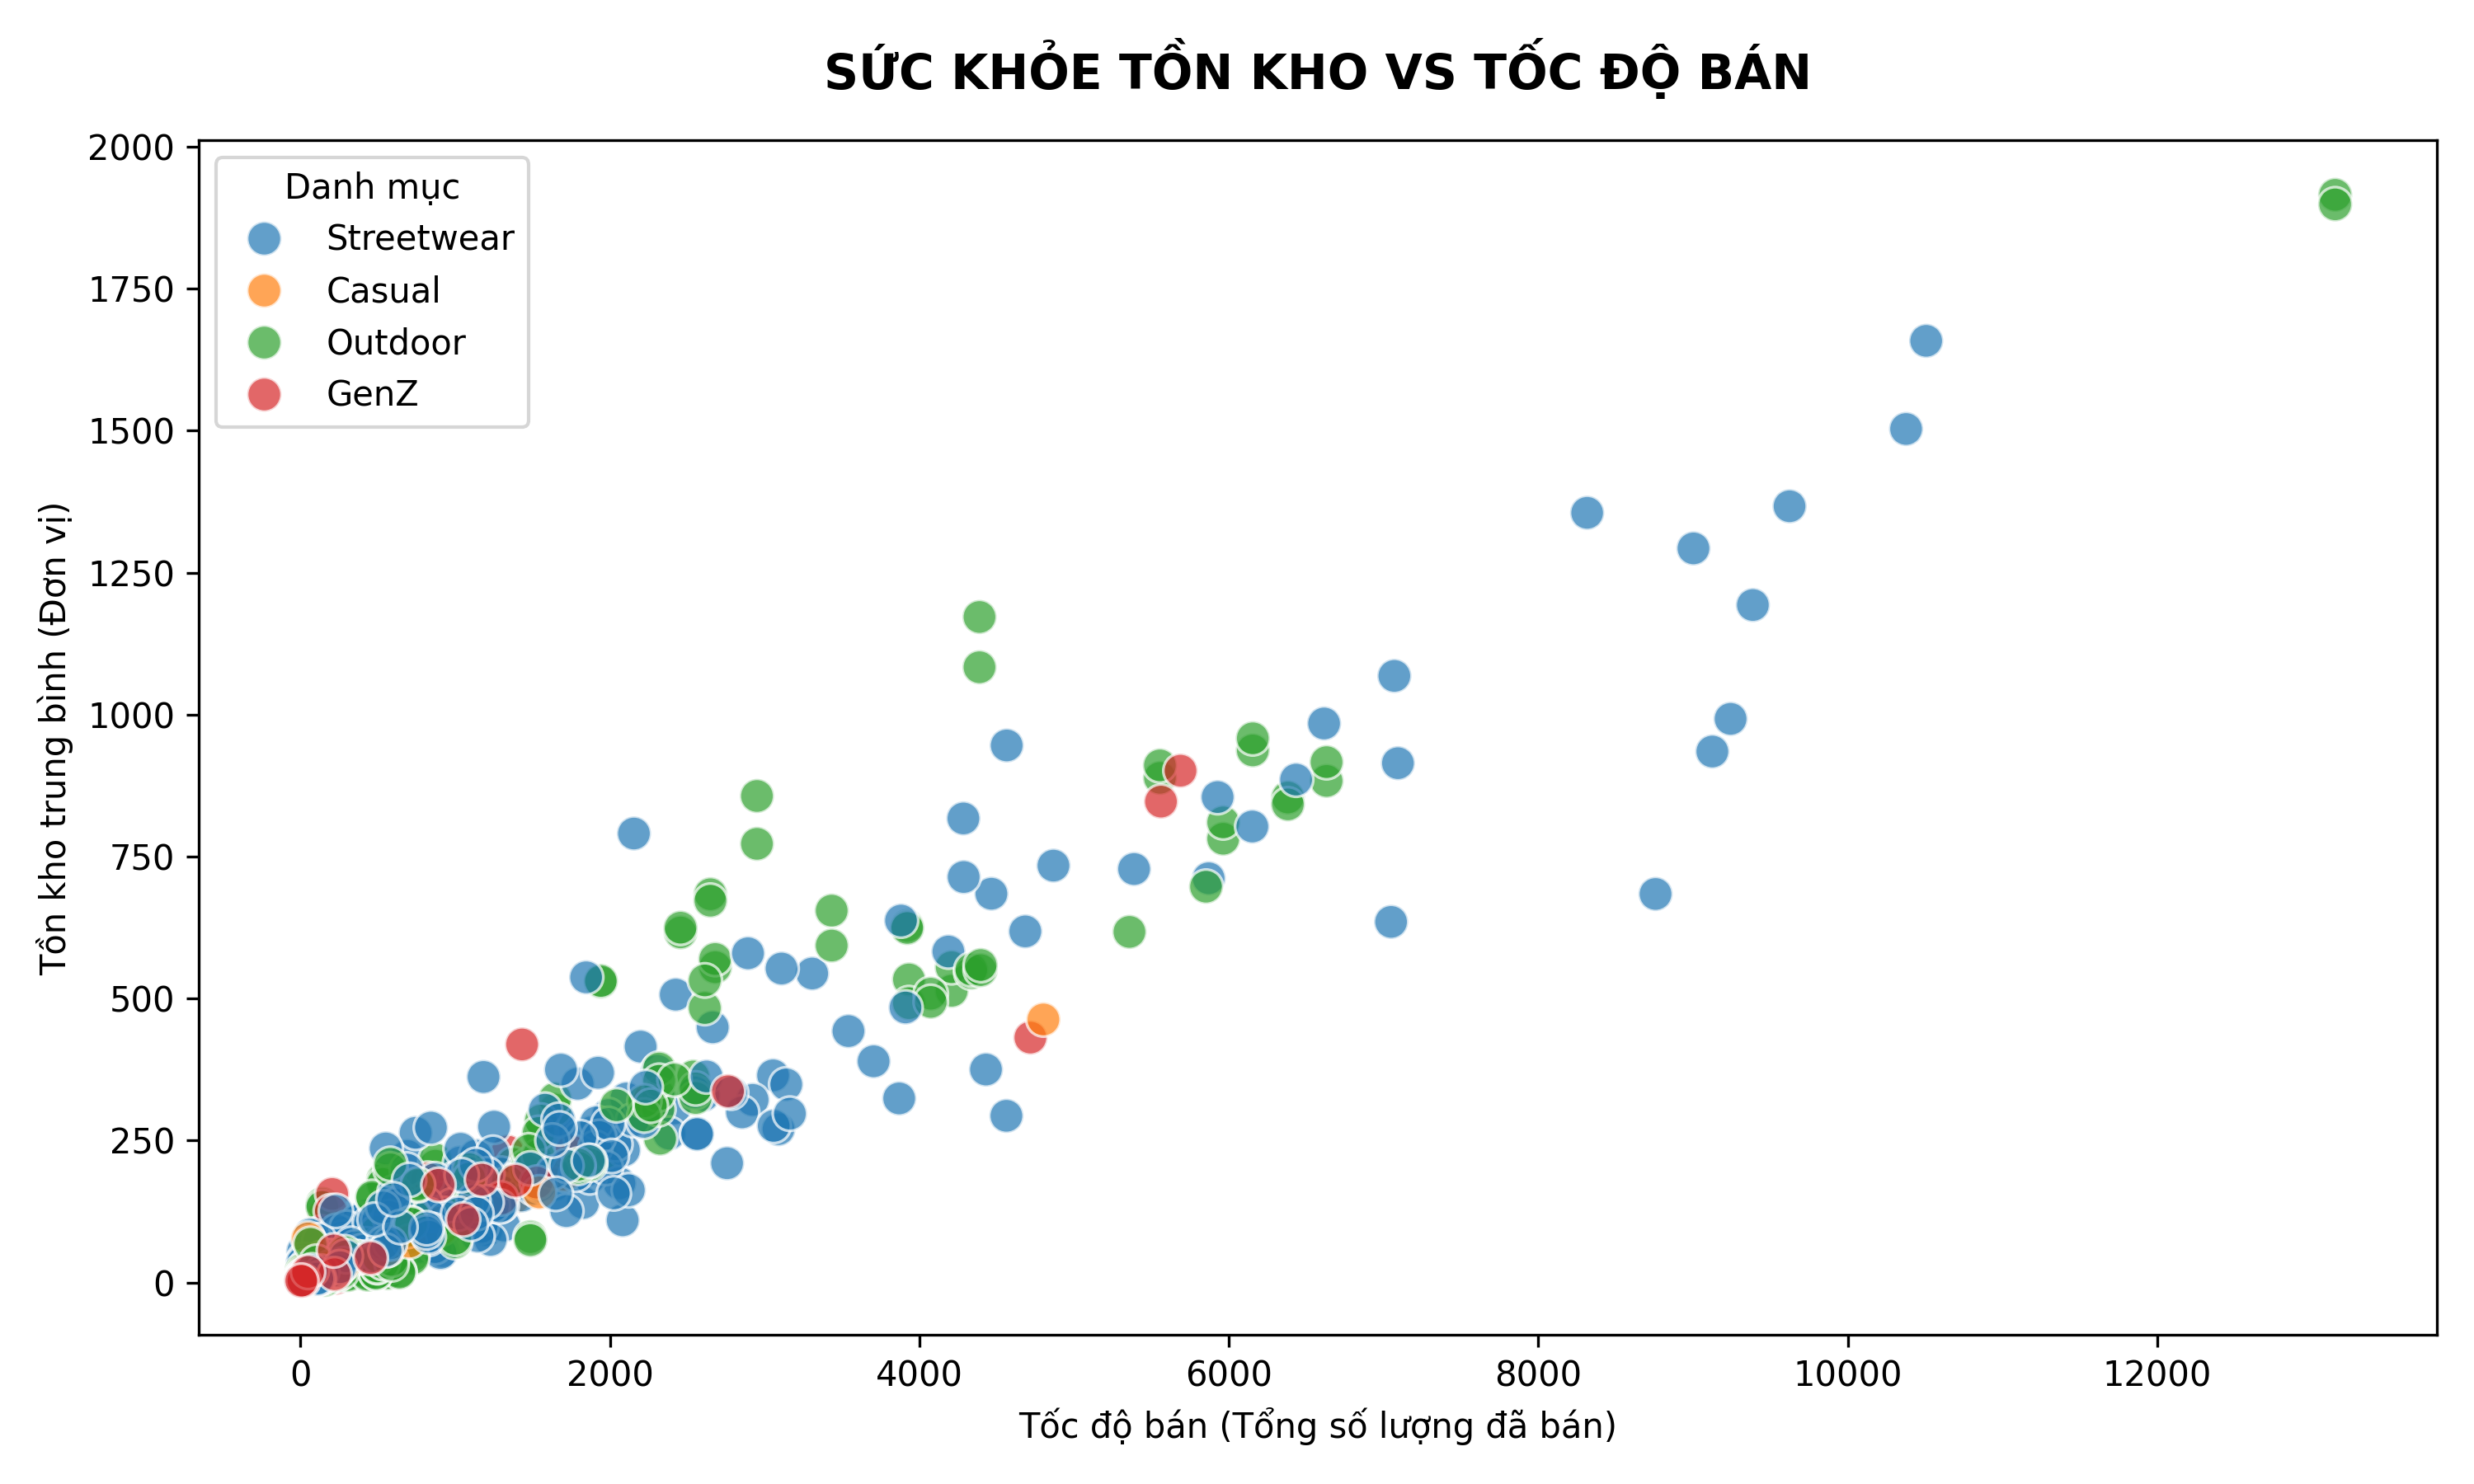
\includegraphics[width=0.48\textwidth]{Images/9b_Inventory_Sales_Velocity.png}
    \caption{(Trái) Ma trận hiệu suất sản phẩm. (Phải) Tốc độ bán vs Tồn kho — Outdoor lệch pha.}
    \label{fig:inventory}
\end{figure}

% ============================================================
\section*{Phần 3 — Mô Hình Dự Báo Doanh Thu}
% ============================================================

\subsection*{Từ Khám Phá Dữ Liệu đến Thiết Kế Dự Báo}

Dựa trên các chẩn đoán (Diagnostic) từ Phần 2, pipeline dự báo được thiết kế chuyên biệt:

\begin{itemize}
    \setlength{\itemsep}{1pt}
    \item \textbf{Khắc phục đứt gãy cấu trúc 2019:} Revenue sụt $-39\%$ phá vỡ tính liên tục xu hướng. Thay vì hồi quy tuyến tính, chúng tôi dùng Tree-based Ensemble kết hợp \textit{Exponential Time-Decay Weighting} $w_t = e^{-0.15(2023 - \text{year}_t)}$, buộc mô hình ưu tiên giai đoạn 2020--2022.
    \item \textbf{Giải quyết dữ liệu khuyết 18 tháng:} Bảng \texttt{promotions}, \texttt{web\_traffic} không tồn tại trong giai đoạn test. Insight mùa vụ từ EDA được mã hóa thành \textit{Fourier Transforms} và \textit{Days-to-Event proxies}, thay thế hoàn toàn External Data.
    \item \textbf{Bảo toàn logic tài chính:} Dự báo COGS gián tiếp qua tỷ lệ $r_t = \text{COGS}/\text{Revenue}$, clip $\in [0.65, 0.95]$, đảm bảo $\text{COGS} \leq \text{Revenue}$ tuyệt đối.
\end{itemize}

\subsection*{Kiến Trúc Pipeline — Hybrid Ensemble}

\textbf{Target transform:} $y = \log(1 + \text{Revenue})$, giảm skewness và ổn định phương sai.

\textbf{Ensemble 18 mô hình} (6 loại $\times$ 3 seeds $[42, 123, 777]$): LightGBM-RMSE (25\%), LightGBM-MAE (10\%), XGBoost-MSE (25\%), CatBoost-RMSE (20\%), CatBoost-MAE (10\%), Random Forest (10\%). Mỗi model chạy 800 rounds, early stopping patience 50.

\textbf{Hybrid Blending:} $90\%$ ML Ensemble $+$ $10\%$ Naive Seasonal Baseline (trung bình Revenue theo \texttt{dayofyear}). Baseline đóng vai trò ``neo'' ổn định, giảm variance tại các ngày ML dự đoán lệch.

\textbf{Trend Multiplier} $\alpha = 1.28$: ML trained trên log-space kết thúc 2022 có xu hướng bám sát mức cũ. Hệ số $\alpha$ bù đắp tăng trưởng:
\[
\hat{R}_t = 1.28 \cdot \left[ 0.9 \cdot \text{expm1}(\hat{y}^{ML}_t) + 0.1 \cdot \hat{y}^{Naive}_t \right], \quad \hat{C}_t = \hat{R}_t \cdot \text{clip}(\hat{r}_t)
\]

\subsection*{Feature Engineering — 41 Đặc Trưng Thuần Thời Gian}

Tất cả features được tạo \textbf{chỉ từ} \texttt{sales\_train.csv} (Date, Revenue, COGS). Không sử dụng dữ liệu ngoài.

\begin{itemize}
    \setlength{\itemsep}{0pt}
    \item \textit{Fourier Transforms} (16): Chu kỳ 365.25 ngày (bậc 1--4), 30.5 ngày (1--2), 7 ngày (1--2) dạng sin/cos.
    \item \textit{Lag đa tầng} (10): DOY-aligned (\texttt{lag\_365}, \texttt{lag\_730}) + DOW-aligned (\texttt{lag\_364}, \texttt{lag\_728}) + COGS lags. Fallback về \texttt{doy\_mean} khi thiếu.
    \item \textit{Seasonal Mean} (4): Trung bình Revenue theo \texttt{dayofyear}, \texttt{weekofyear}, tháng, thứ.
    \item \textit{Calendar} (11): \texttt{time\_idx}, payday, double\_day, month\_end, weekend, interactions.
\end{itemize}

\subsection*{Xác Thực Chéo Theo Thời Gian (Temporal Validation)}

Để mô phỏng khoảng trống 18 tháng của tập Test và triệt tiêu Look-ahead Bias:

\begin{itemize}
    \setlength{\itemsep}{1pt}
    \item \textbf{Tập Train:} 04/07/2012 -- 30/06/2021 (9 năm, 3.284 ngày).
    \item \textbf{Tập Validation:} 01/07/2021 -- 31/12/2022 (\textbf{549 ngày} — tương đương tập Test).
\end{itemize}

Không sử dụng random split. Revenue/COGS từ tập test \textbf{không bao giờ} xuất hiện trong features hay quá trình huấn luyện. Lag features cho 2024 tự động fallback về seasonal means.

\subsection*{Kết Quả Thực Nghiệm}

\begin{table}[H]
\centering
\small
\caption{Hiệu suất mô hình — Hold-out Validation \& Public Leaderboard}
\label{tab:metrics}
\begin{tabular}{lcccc}
\toprule
\textbf{Mô hình} & \textbf{Val RMSE} & \textbf{Val MAE} & \textbf{Val $R^2$} & \textbf{LB RMSE} \\
\midrule
Naive Baseline & 912K & 724K & 0.41 & $>$900K \\
LightGBM đơn (V37) & 699K & 531K & 0.80 & 780K \\
\textbf{V55 Ensemble} & \textbf{685K} & \textbf{512K} & \textbf{0.81} & \textbf{740.8K} \\
V58 Deep Trees & 701K & 538K & 0.79 & 743K \\
V60 Ridge Hybrid & 728K & 569K & 0.76 & 769K \\
\bottomrule
\end{tabular}
\end{table}

\textbf{Sanity checks:} 0 giá trị âm Revenue, 0 vi phạm $\text{COGS} > \text{Revenue}$, dự báo 2023--2024 tăng trưởng $+27\%$ (phù hợp xu hướng phục hồi kinh tế hậu COVID).

\subsection*{Giải Thích Mô Hình — SHAP Analysis}

SHAP TreeExplainer xác nhận các proxy thời gian đã hoàn toàn thống trị dự báo, thay thế an toàn cho dữ liệu External:

\begin{enumerate}
    \setlength{\itemsep}{1pt}
    \item \textbf{Seasonal Mean:} \texttt{rev\_doy\_mean} (SHAP \#1) — mô hình học rằng doanh thu mỗi ngày bám sát trung bình lịch sử cùng ngày trong năm.
    \item \textbf{Xu hướng:} \texttt{time\_idx} (SHAP \#2) — nhờ decay weighting, mô hình phân biệt giai đoạn cũ vs mới.
    \item \textbf{Quán tính thường niên:} \texttt{rev\_lag\_365/730} (SHAP \#3--5) — doanh thu cùng kỳ là anchor cực mạnh.
\end{enumerate}

\begin{figure}[H]
    \centering
    \begin{subfigure}{0.48\textwidth}
        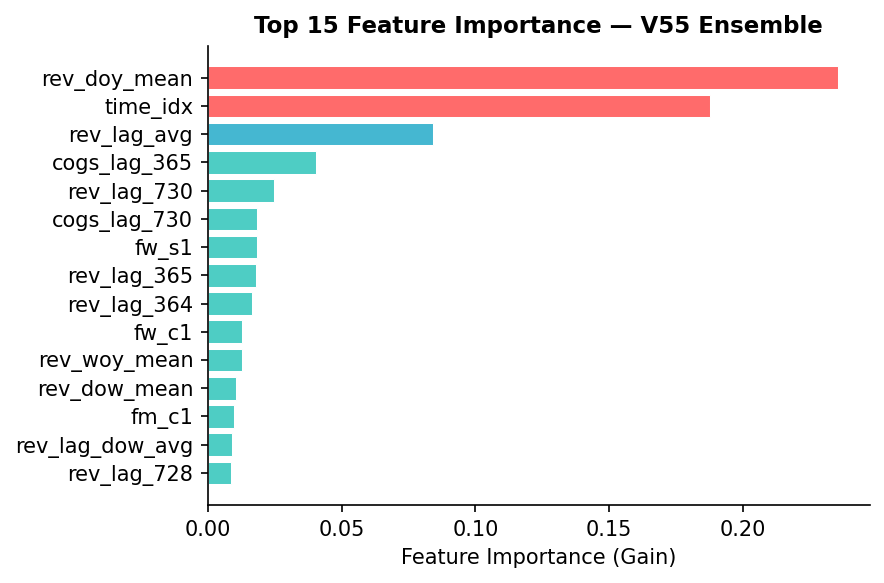
\includegraphics[width=\linewidth]{Images/shap_bar_v55.png}
        \caption{Feature Importance (Gain)}
    \end{subfigure}
    \hfill
    \begin{subfigure}{0.48\textwidth}
        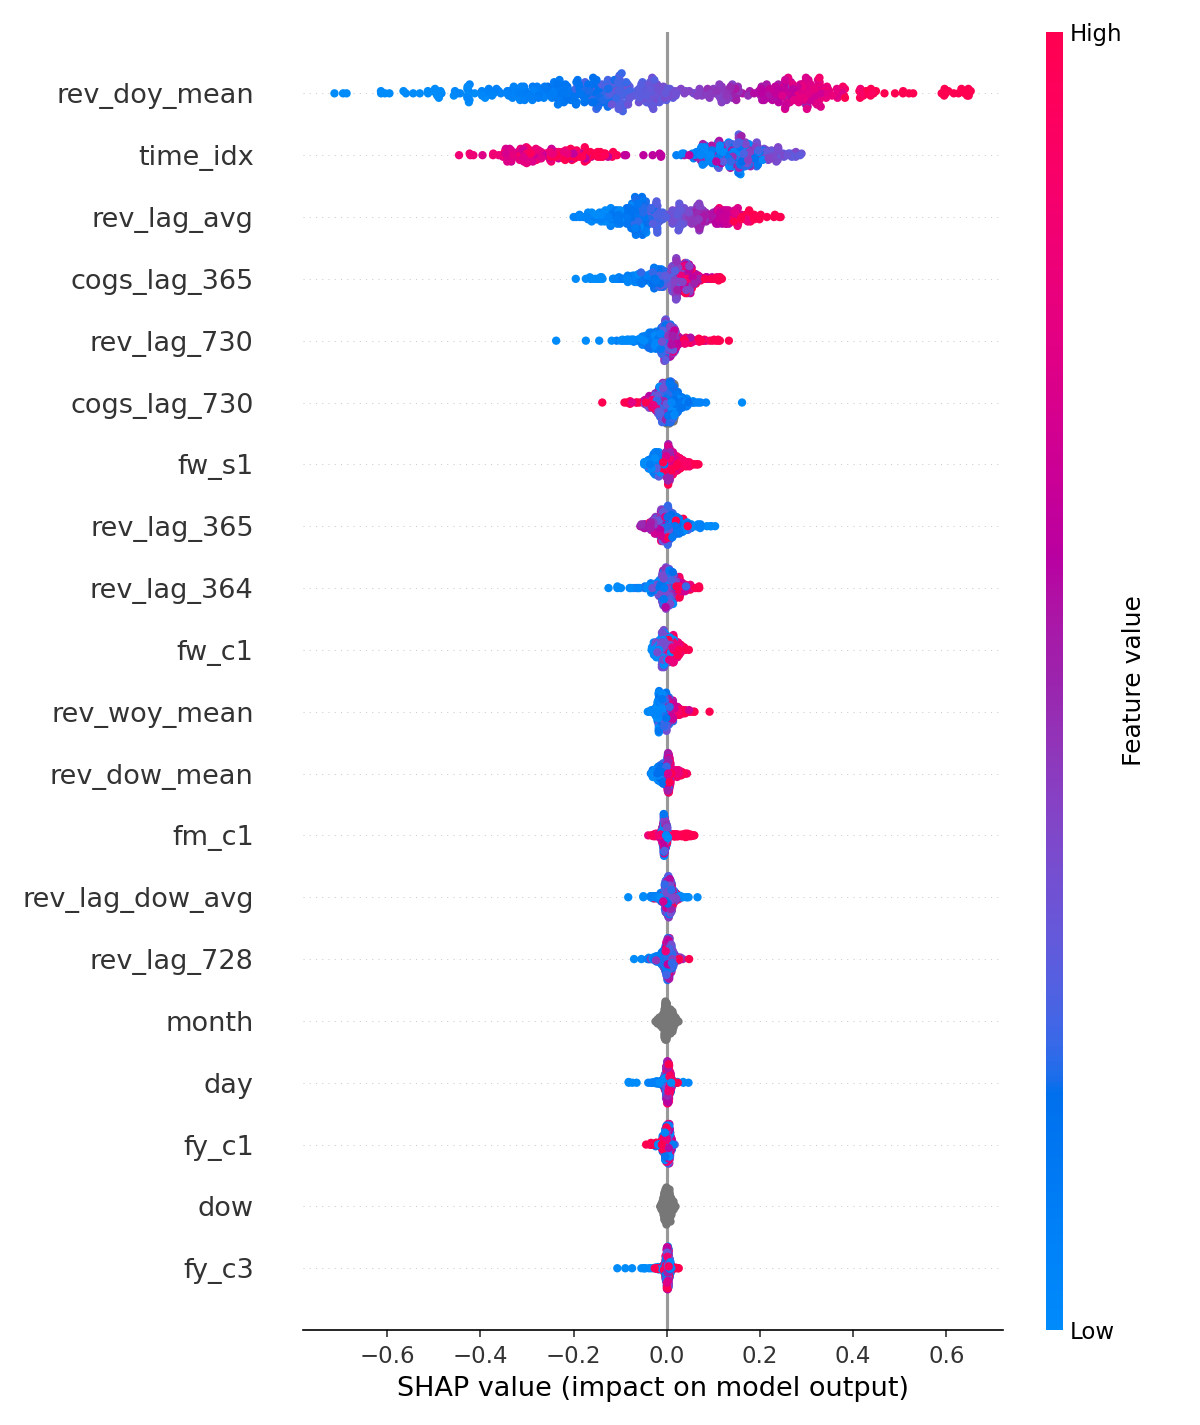
\includegraphics[width=\linewidth]{Images/shap_beeswarm_v55.png}
        \caption{SHAP Beeswarm — phân bổ tác động}
    \end{subfigure}
    \vspace{-0.2cm}
    \caption{Explainability: Fourier/Lag proxies thống trị dự báo, thay thế hoàn toàn External Data.}
    \label{fig:shap}
\end{figure}

% ============================================================
\section*{Chiến Lược Thực Thi \& Kết Luận}
% ============================================================

Để giải quyết 4 điểm nghẽn, chúng tôi đề xuất 5 trụ cột hành động:

\begin{enumerate}
    \setlength{\itemsep}{2pt}
    \item \textbf{Tái cấu trúc Khuyến mãi:} Cross-selling ``Mua 1 Streetwear nguyên giá — Outdoor giảm $70\%$'', tận dụng Cash Cow thanh lý tồn kho.
    \item \textbf{Tối ưu Mobile Checkout:} Tích hợp BNPL ngay trang sản phẩm, phá rào cản tâm lý giá mà không cắt biên lợi nhuận.
    \item \textbf{Tái phân bổ vốn:} Đóng băng 3 SKU deadstock, chuyển $100\%$ dòng tiền sang Streetwear.
    \item \textbf{Chuyển dịch tiếp thị:} Dịch chuyển từ HN/HCM bão hòa sang thị trường Cấp 2 qua SEO/Email.
    \item \textbf{Nâng Safety Stock trước Double Day:} \textbf{Đánh đổi:} Holding Cost tăng $\sim$2\%, nhưng dựa trên năng lực dự báo (RMSE 740.8K), ước tính cứu vãn \textbf{12\% Lost Sales} do Stockout.
\end{enumerate}

\textbf{KPI mục tiêu:} Gross Margin $+20\%$, AOV 27.500 VNĐ ($+25\%$), Outdoor Overstock $80\% \to 40\%$, Mobile Abandonment $<40\%$.

\textbf{Tái lập kết quả:}\footnote{Phần 1 (Trắc nghiệm) được nộp riêng qua Biểu mẫu. Báo cáo này tập trung Phần 2 và Phần 3.}

{\small\texttt{pip install -r requirements.txt \&\& python scripts/train\_v55\_ultimate.py}}

\noindent Công khai tại: \url{https://github.com/DuongNAD/datathon-2026-submission}. Seeds: $[42, 123, 777]$. Tái lập 100\%.

% ============================================================
% REFERENCES (không tính vào 4 trang)
% ============================================================
\newpage
\section*{Tài liệu tham khảo}

\begin{enumerate}
    \setlength{\itemsep}{2pt}
    \item Ke, G., et al. ``LightGBM: A Highly Efficient Gradient Boosting Decision Tree.'' \textit{NeurIPS}, 2017.
    \item Chen, T. \& Guestrin, C. ``XGBoost: A Scalable Tree Boosting System.'' \textit{KDD}, 2016.
    \item Prokhorenkova, L., et al. ``CatBoost: Unbiased Boosting with Categorical Features.'' \textit{NeurIPS}, 2018.
    \item Lundberg, S. M. \& Lee, S.-I. ``A Unified Approach to Interpreting Model Predictions (SHAP).'' \textit{NeurIPS}, 2017.
    \item VinTelligence — VinUniversity DS\&AI Club. ``Đề thi Datathon 2026 — Vòng 1: The Gridbreakers.'' 2026.
\end{enumerate}

% ============================================================
% APPENDIX (không tính vào 4 trang)
% ============================================================
\section*{Phụ lục}

\begin{figure}[H]
    \centering
    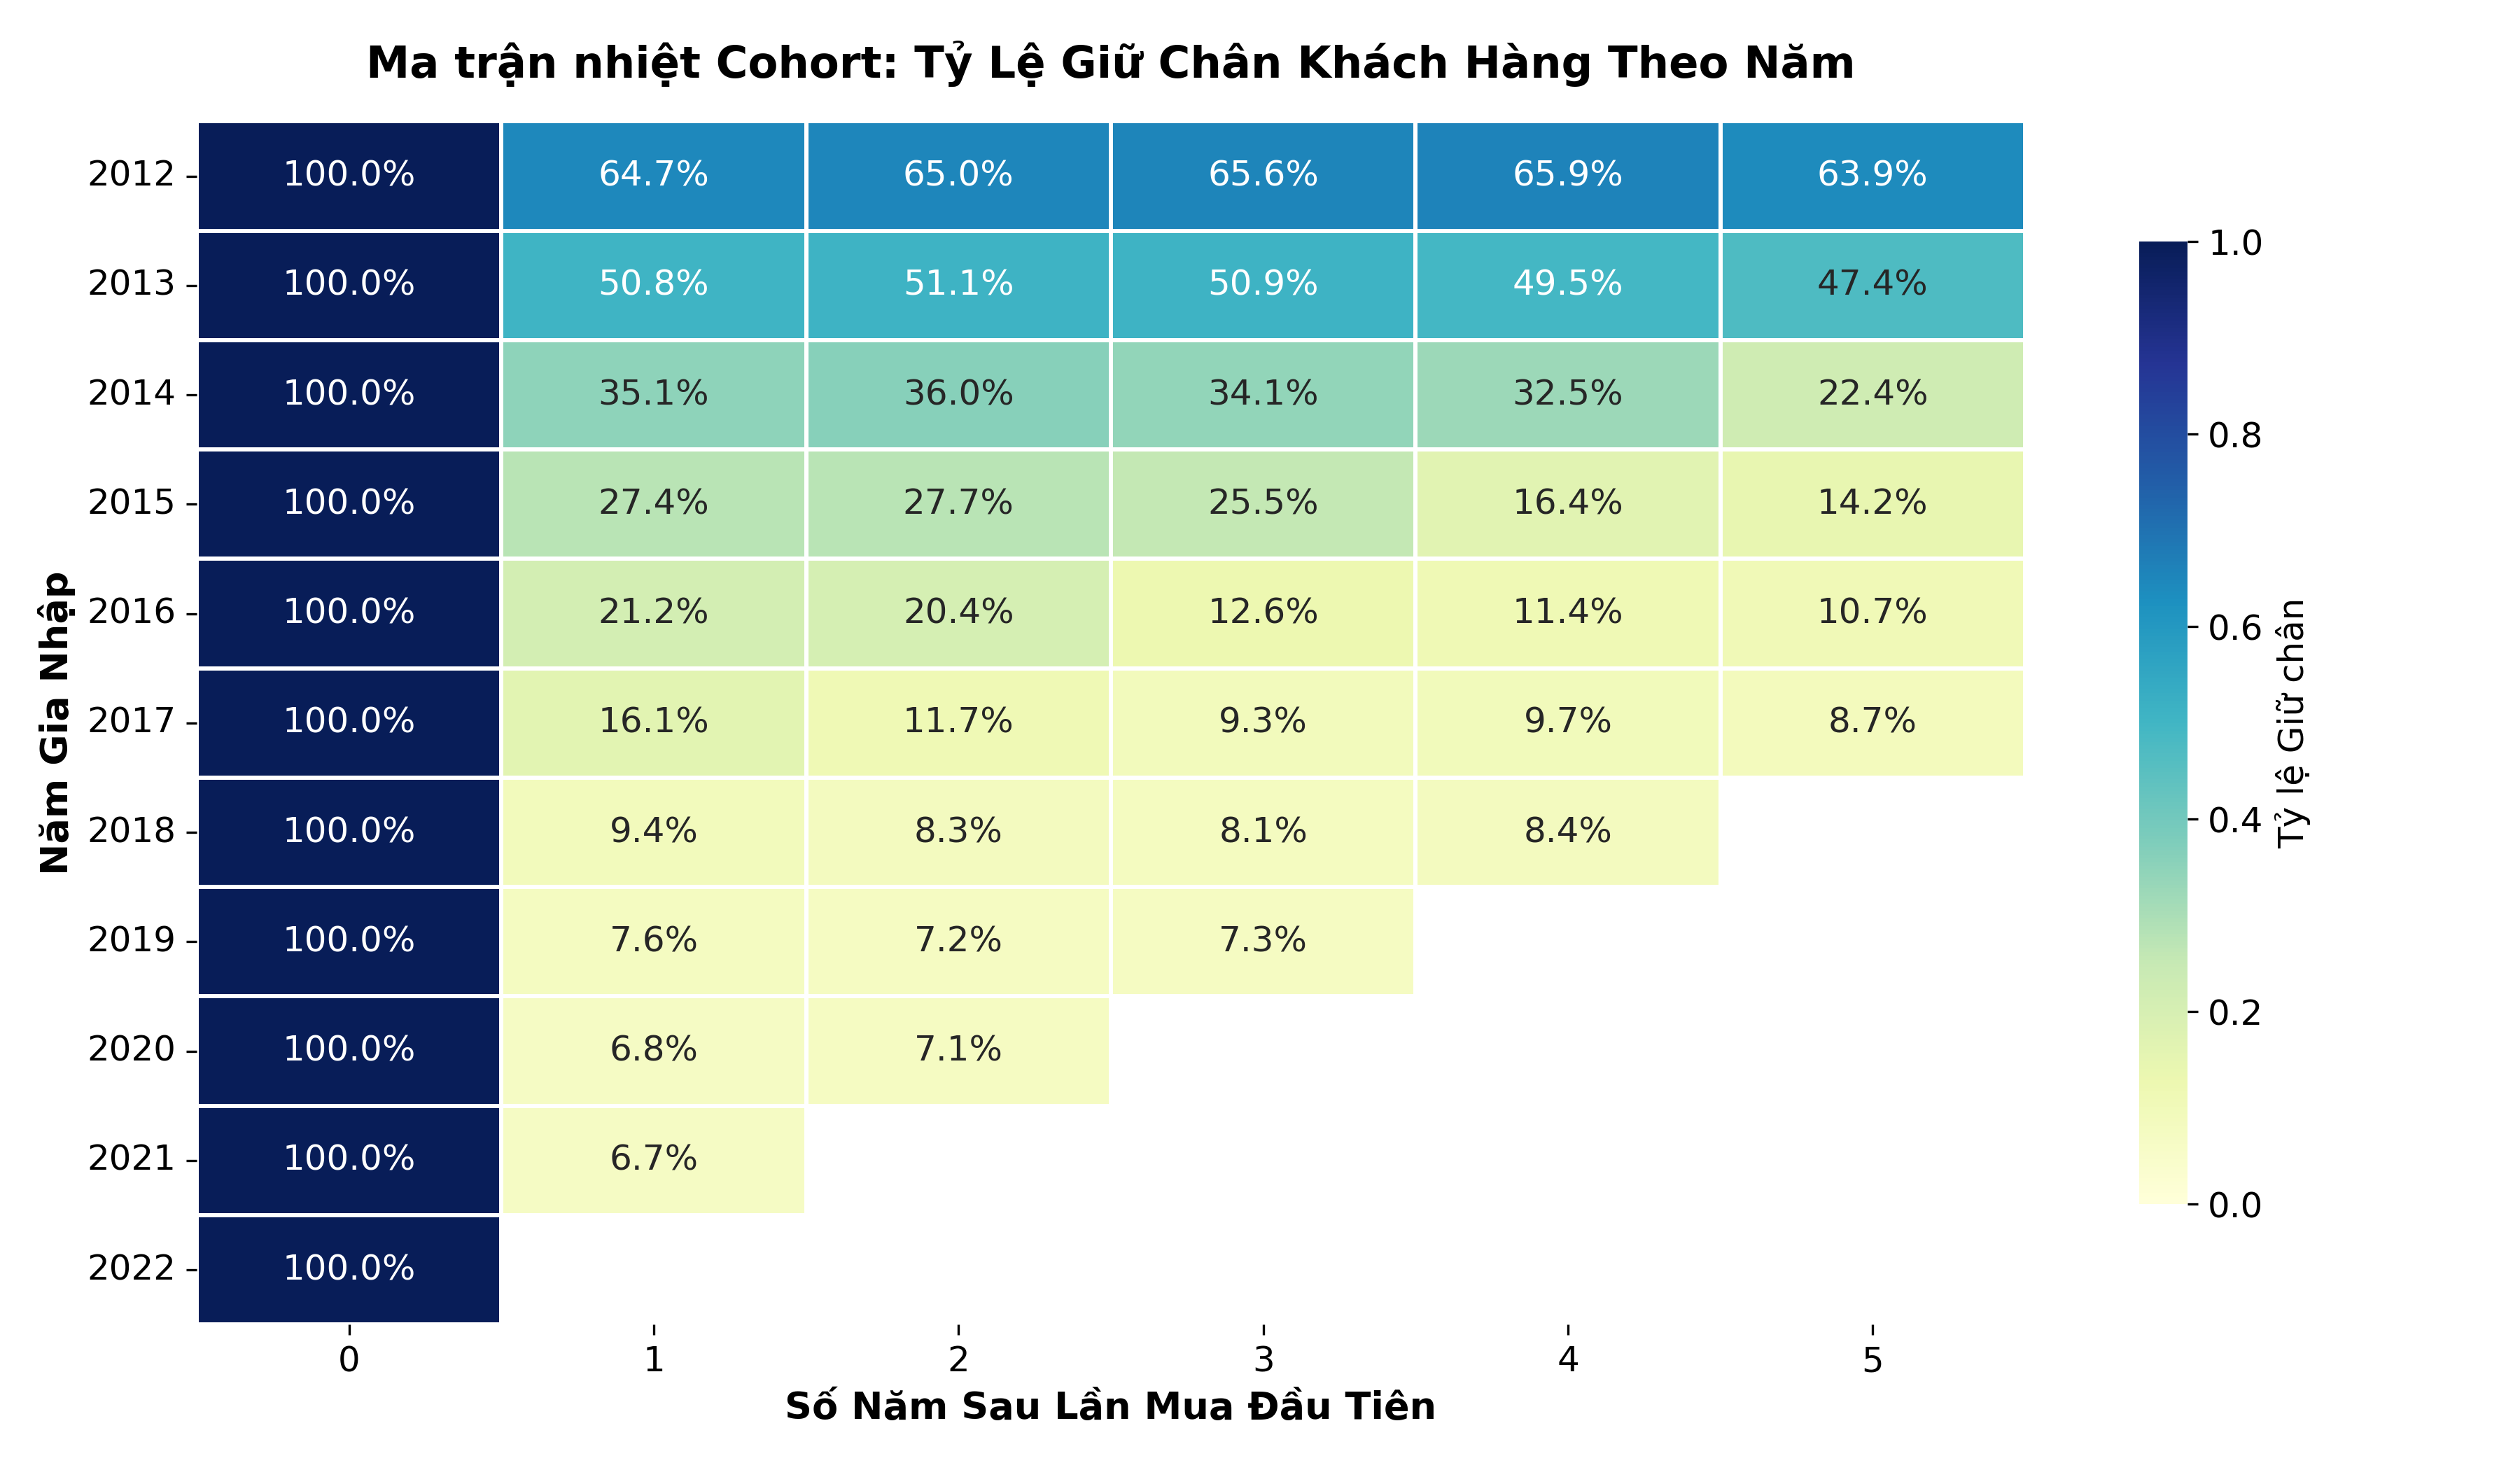
\includegraphics[width=0.48\textwidth]{Images/10a_Cohort_Heatmap.png}
    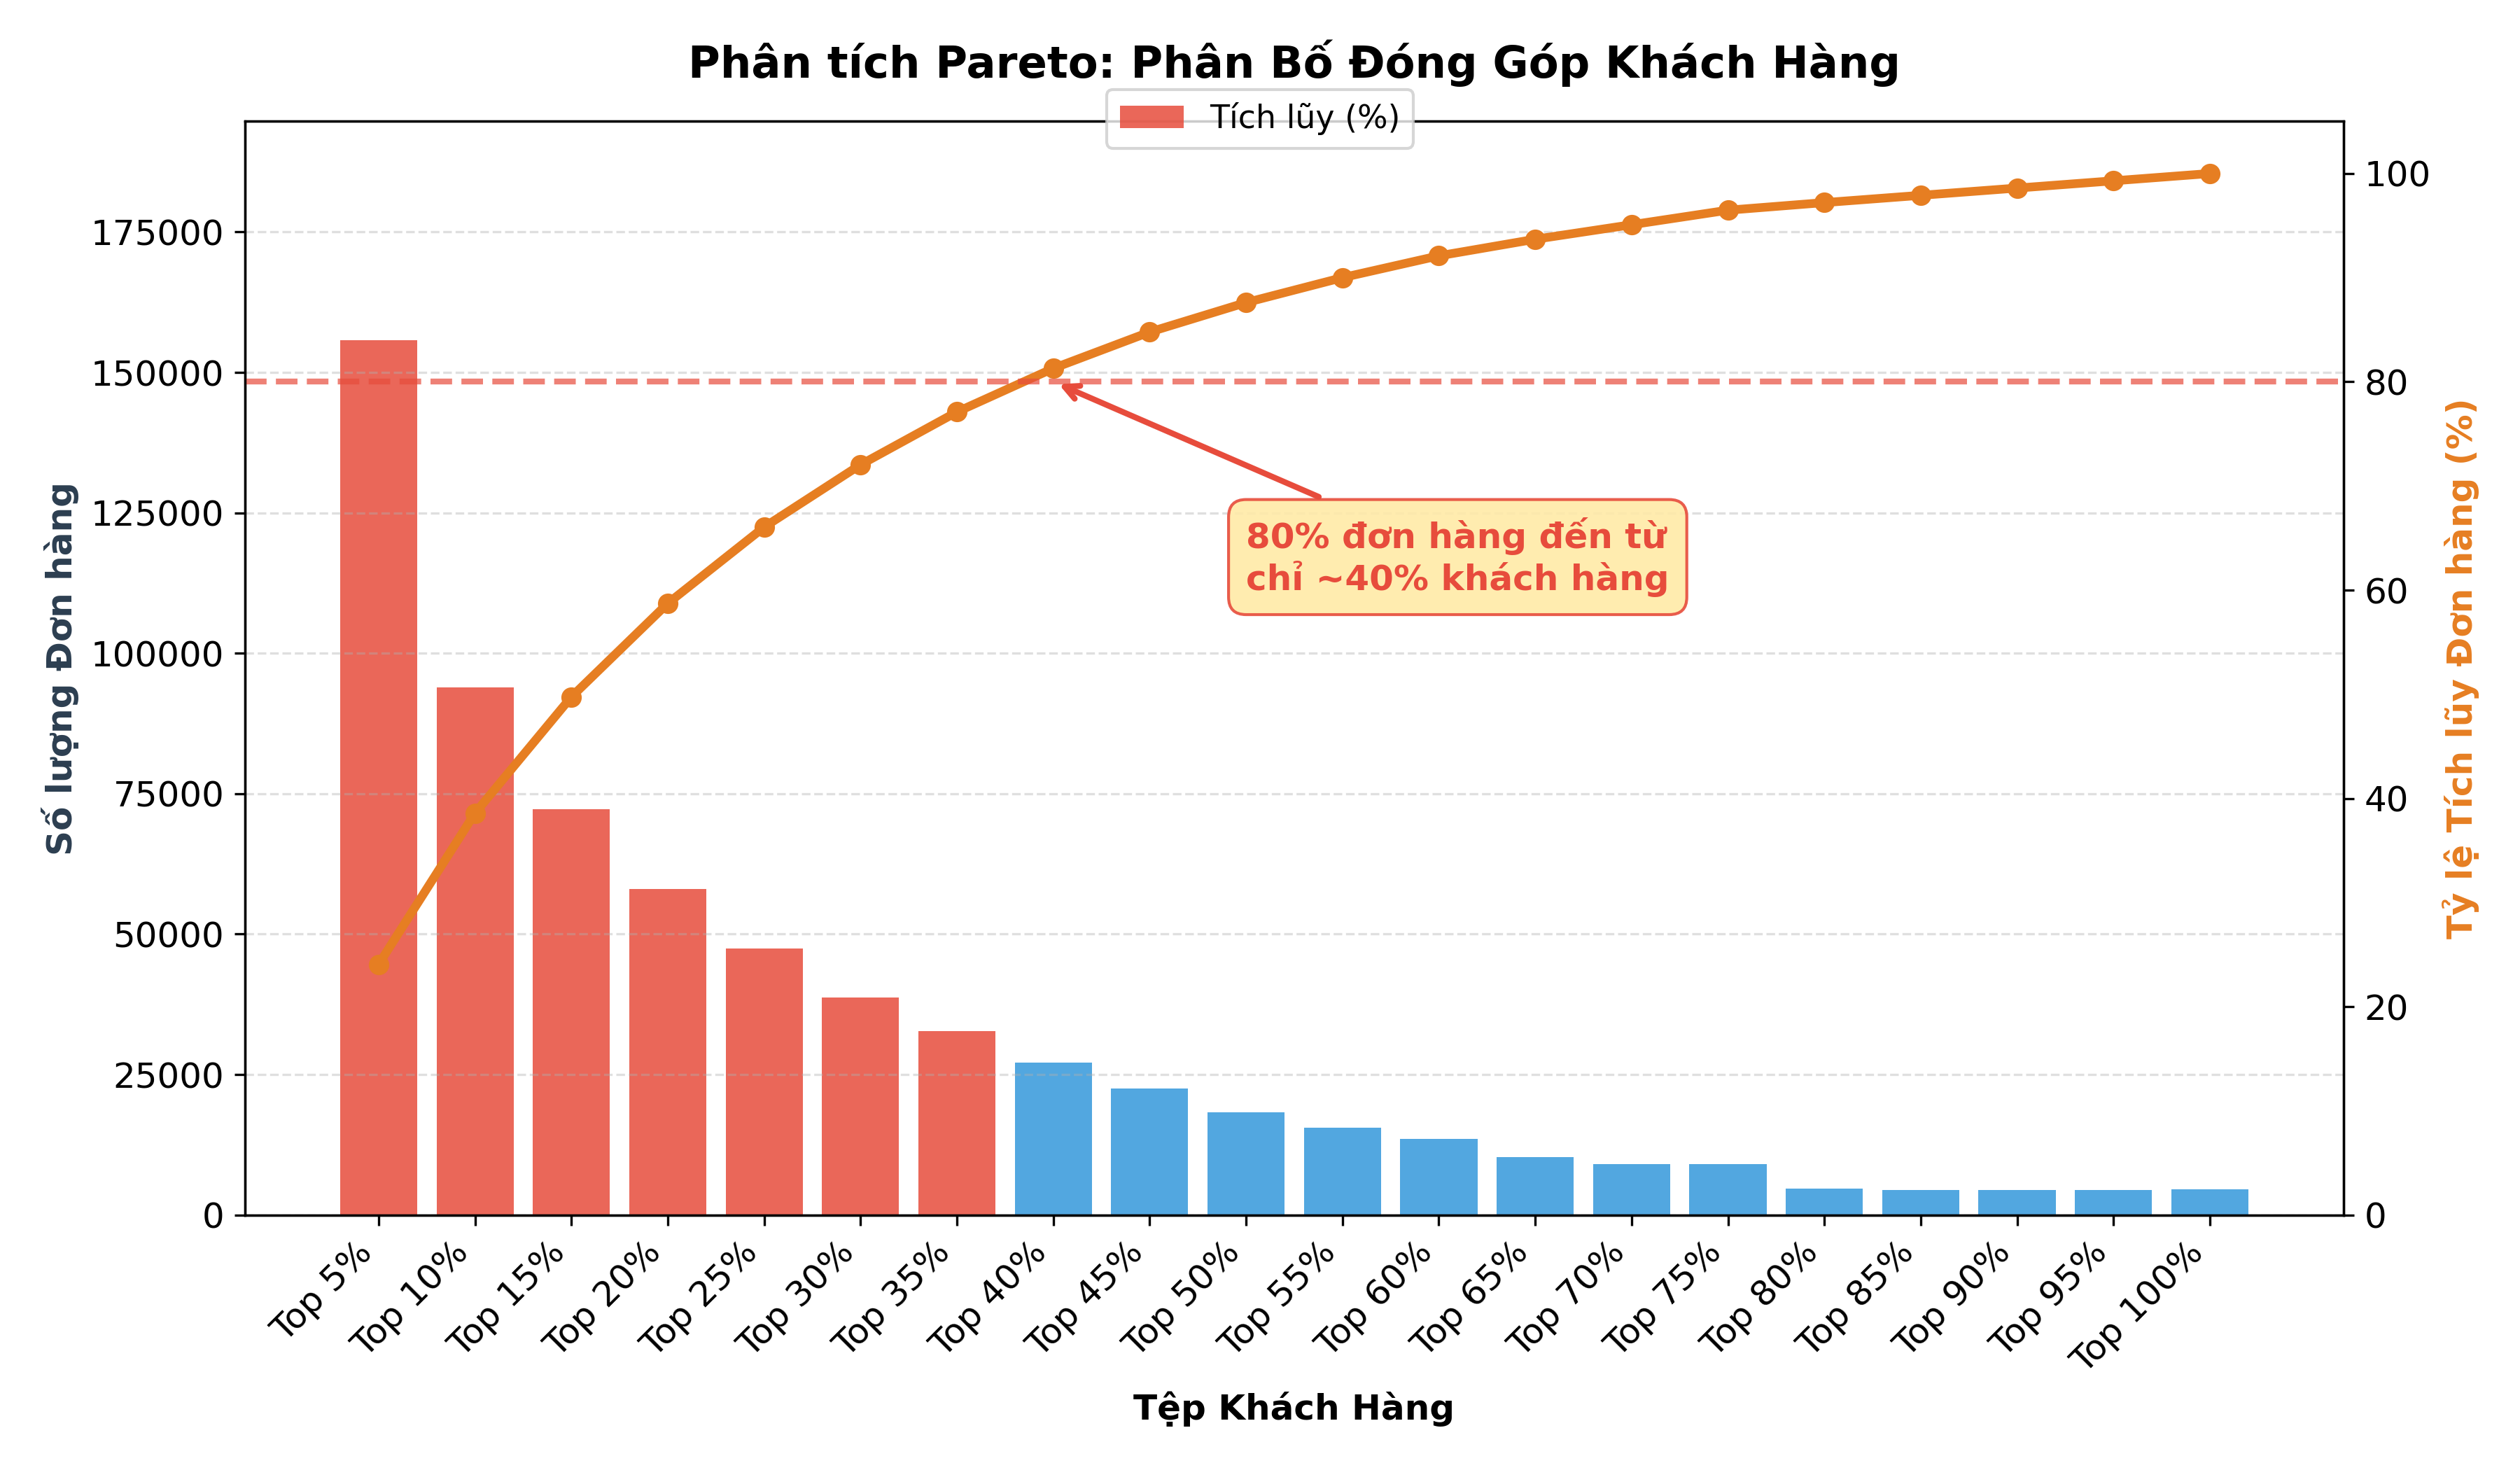
\includegraphics[width=0.48\textwidth]{Images/10b_Pareto_Chart.png}
    \caption{(Trái) Cohort Heatmap — tỷ lệ giữ chân sụt mạnh Năm 0 $\rightarrow$ Năm 1. (Phải) Pareto — Top $40\%$ KH đóng góp $80\%$ tổng đơn.}
    \label{fig:appendix1}
\end{figure}

\begin{figure}[H]
    \centering
    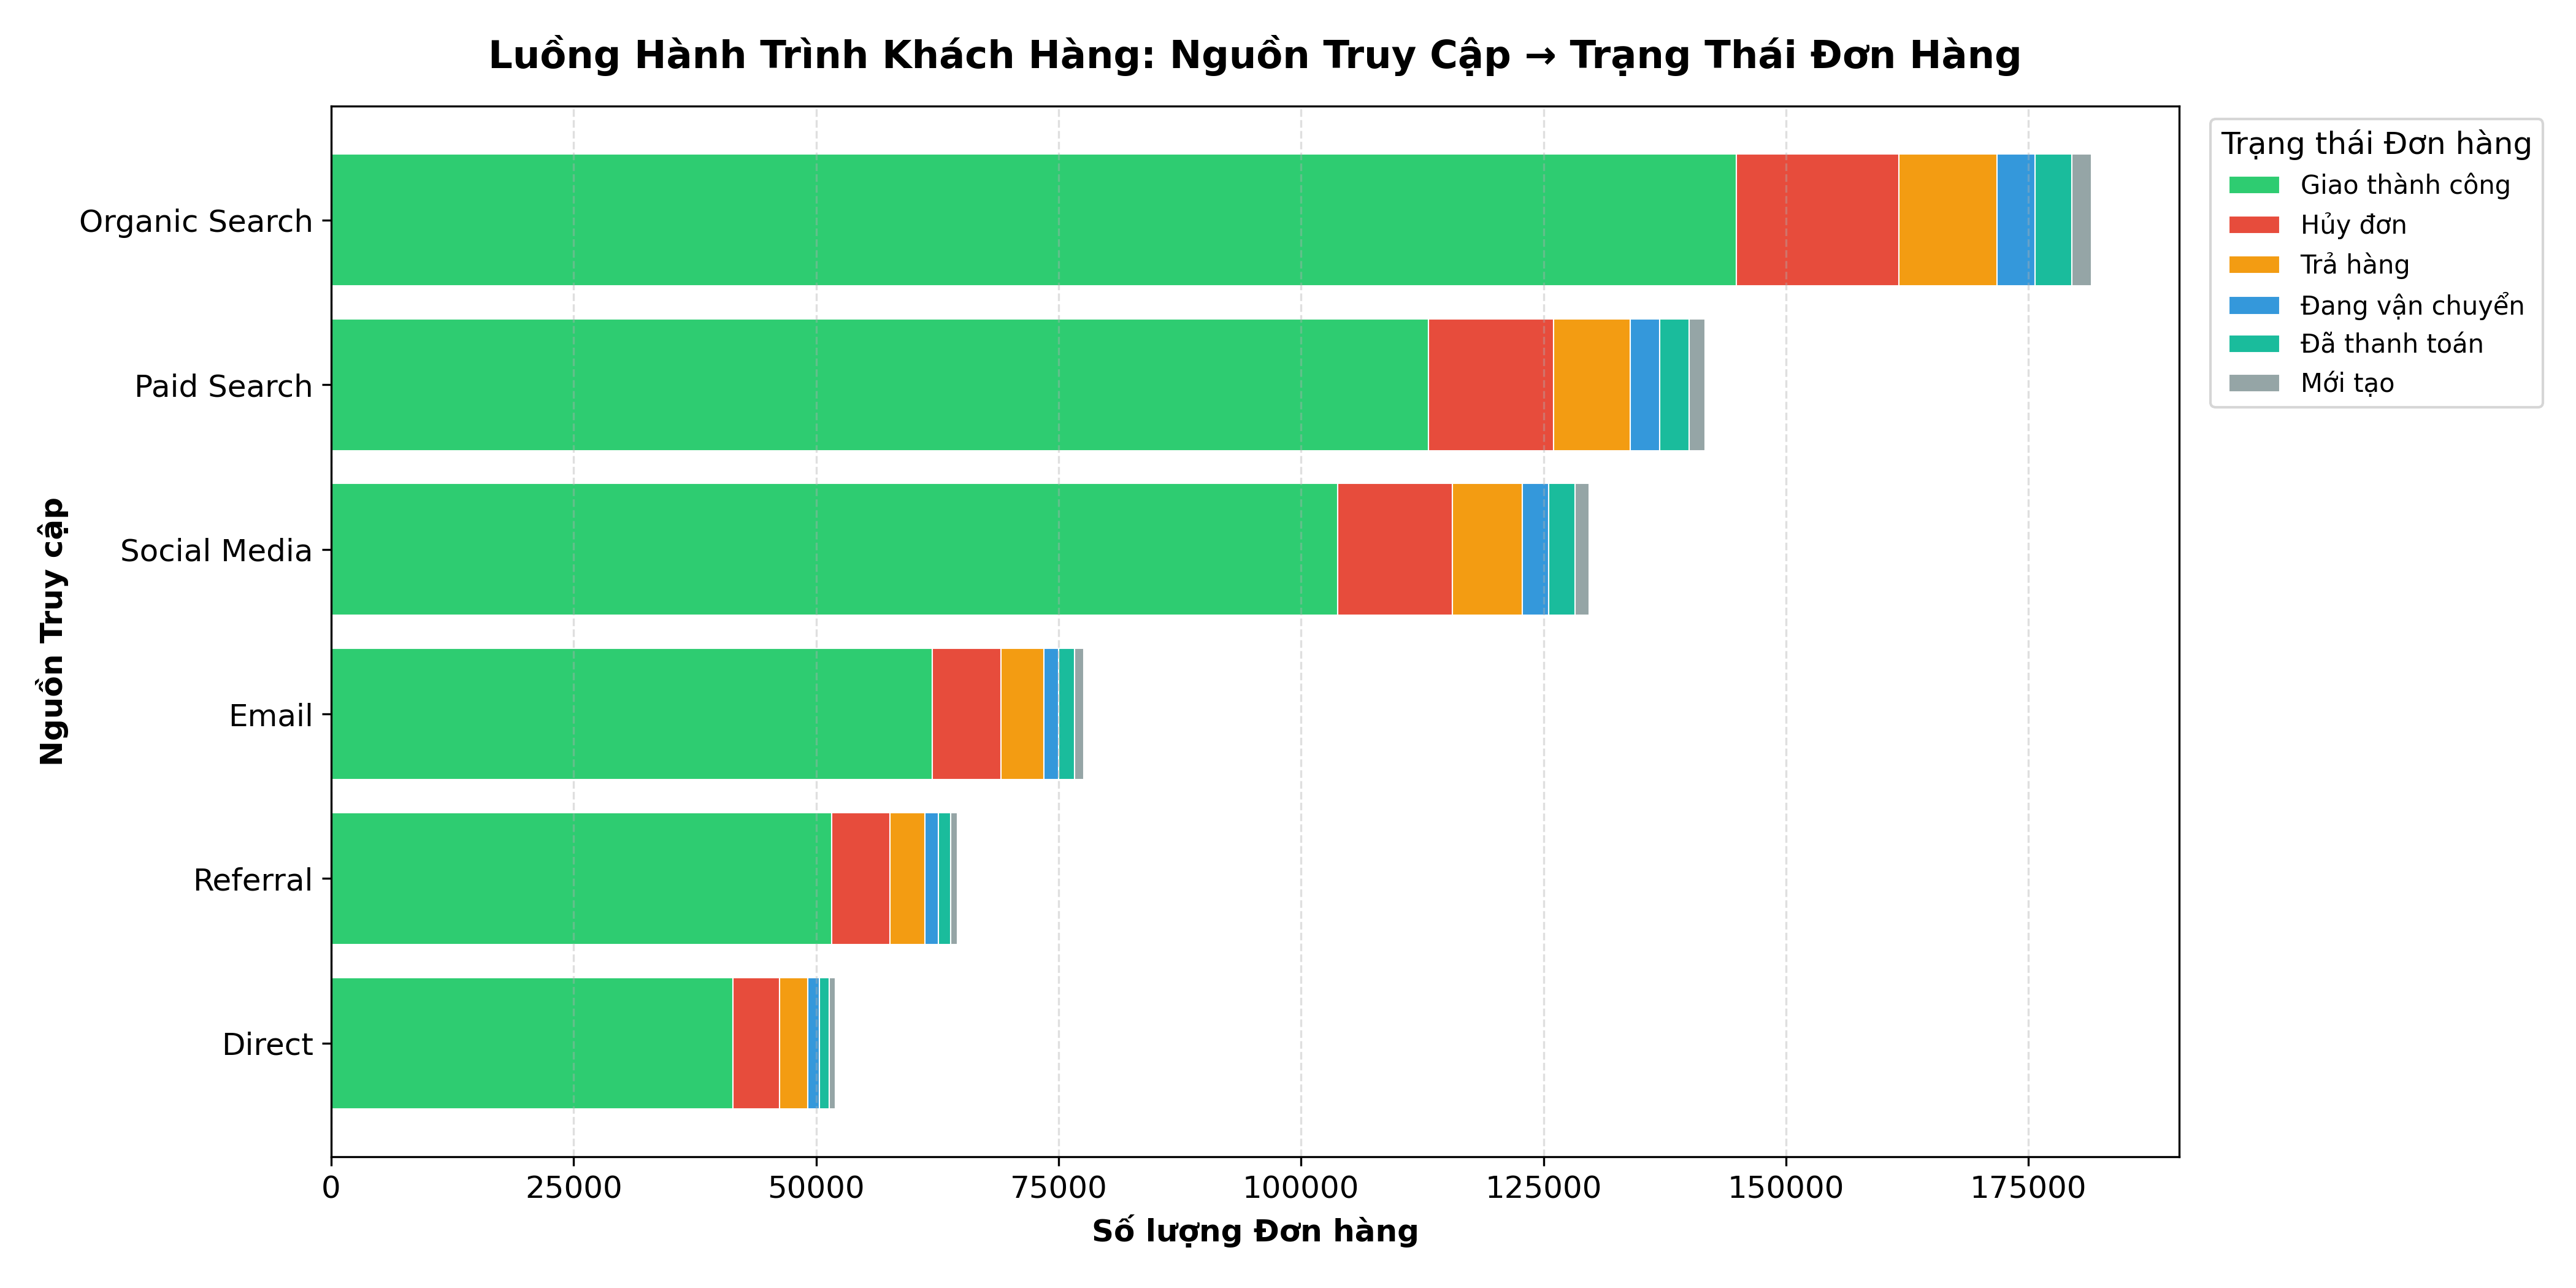
\includegraphics[width=0.48\textwidth]{Images/10c_Sankey_Diagram.png}
    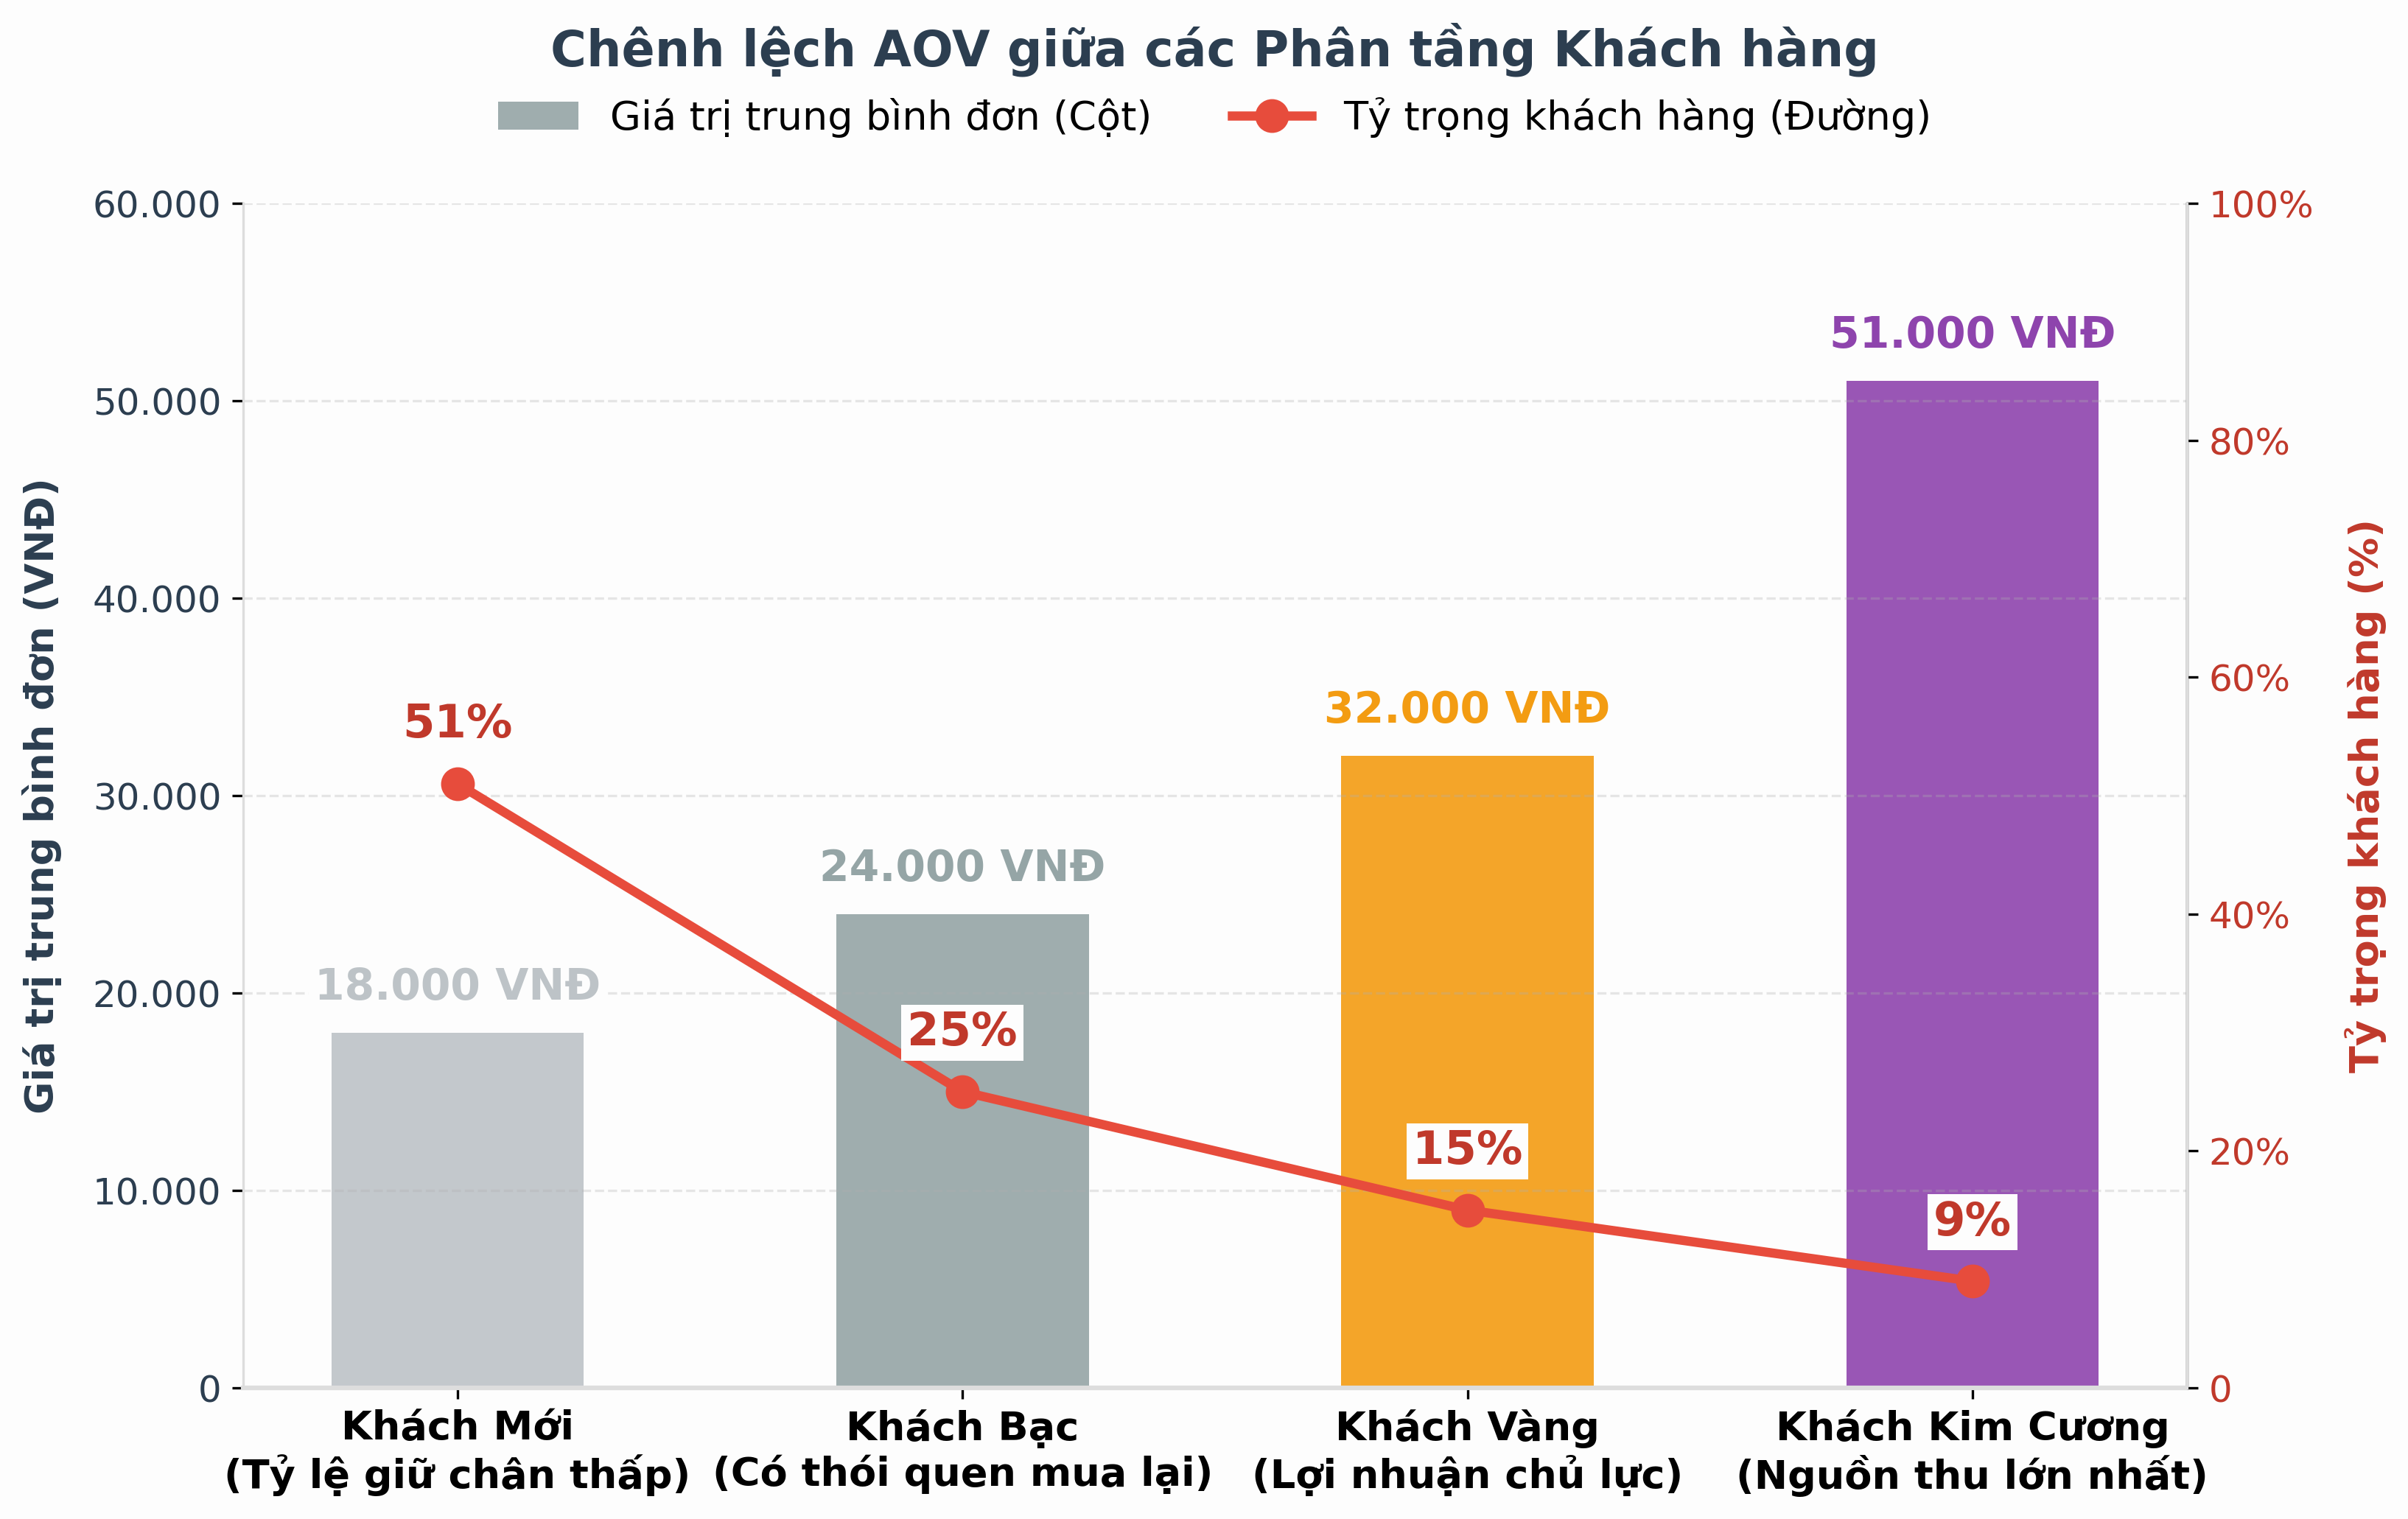
\includegraphics[width=0.48\textwidth]{Images/8_Customer_Tier_Behavior.png}
    \caption{(Trái) Sankey — luồng hành trình khách hàng. (Phải) Chênh lệch AOV giữa phân tầng — VIP $9\%$ chi phối dòng tiền.}
    \label{fig:appendix2}
\end{figure}

\begin{figure}[H]
    \centering
    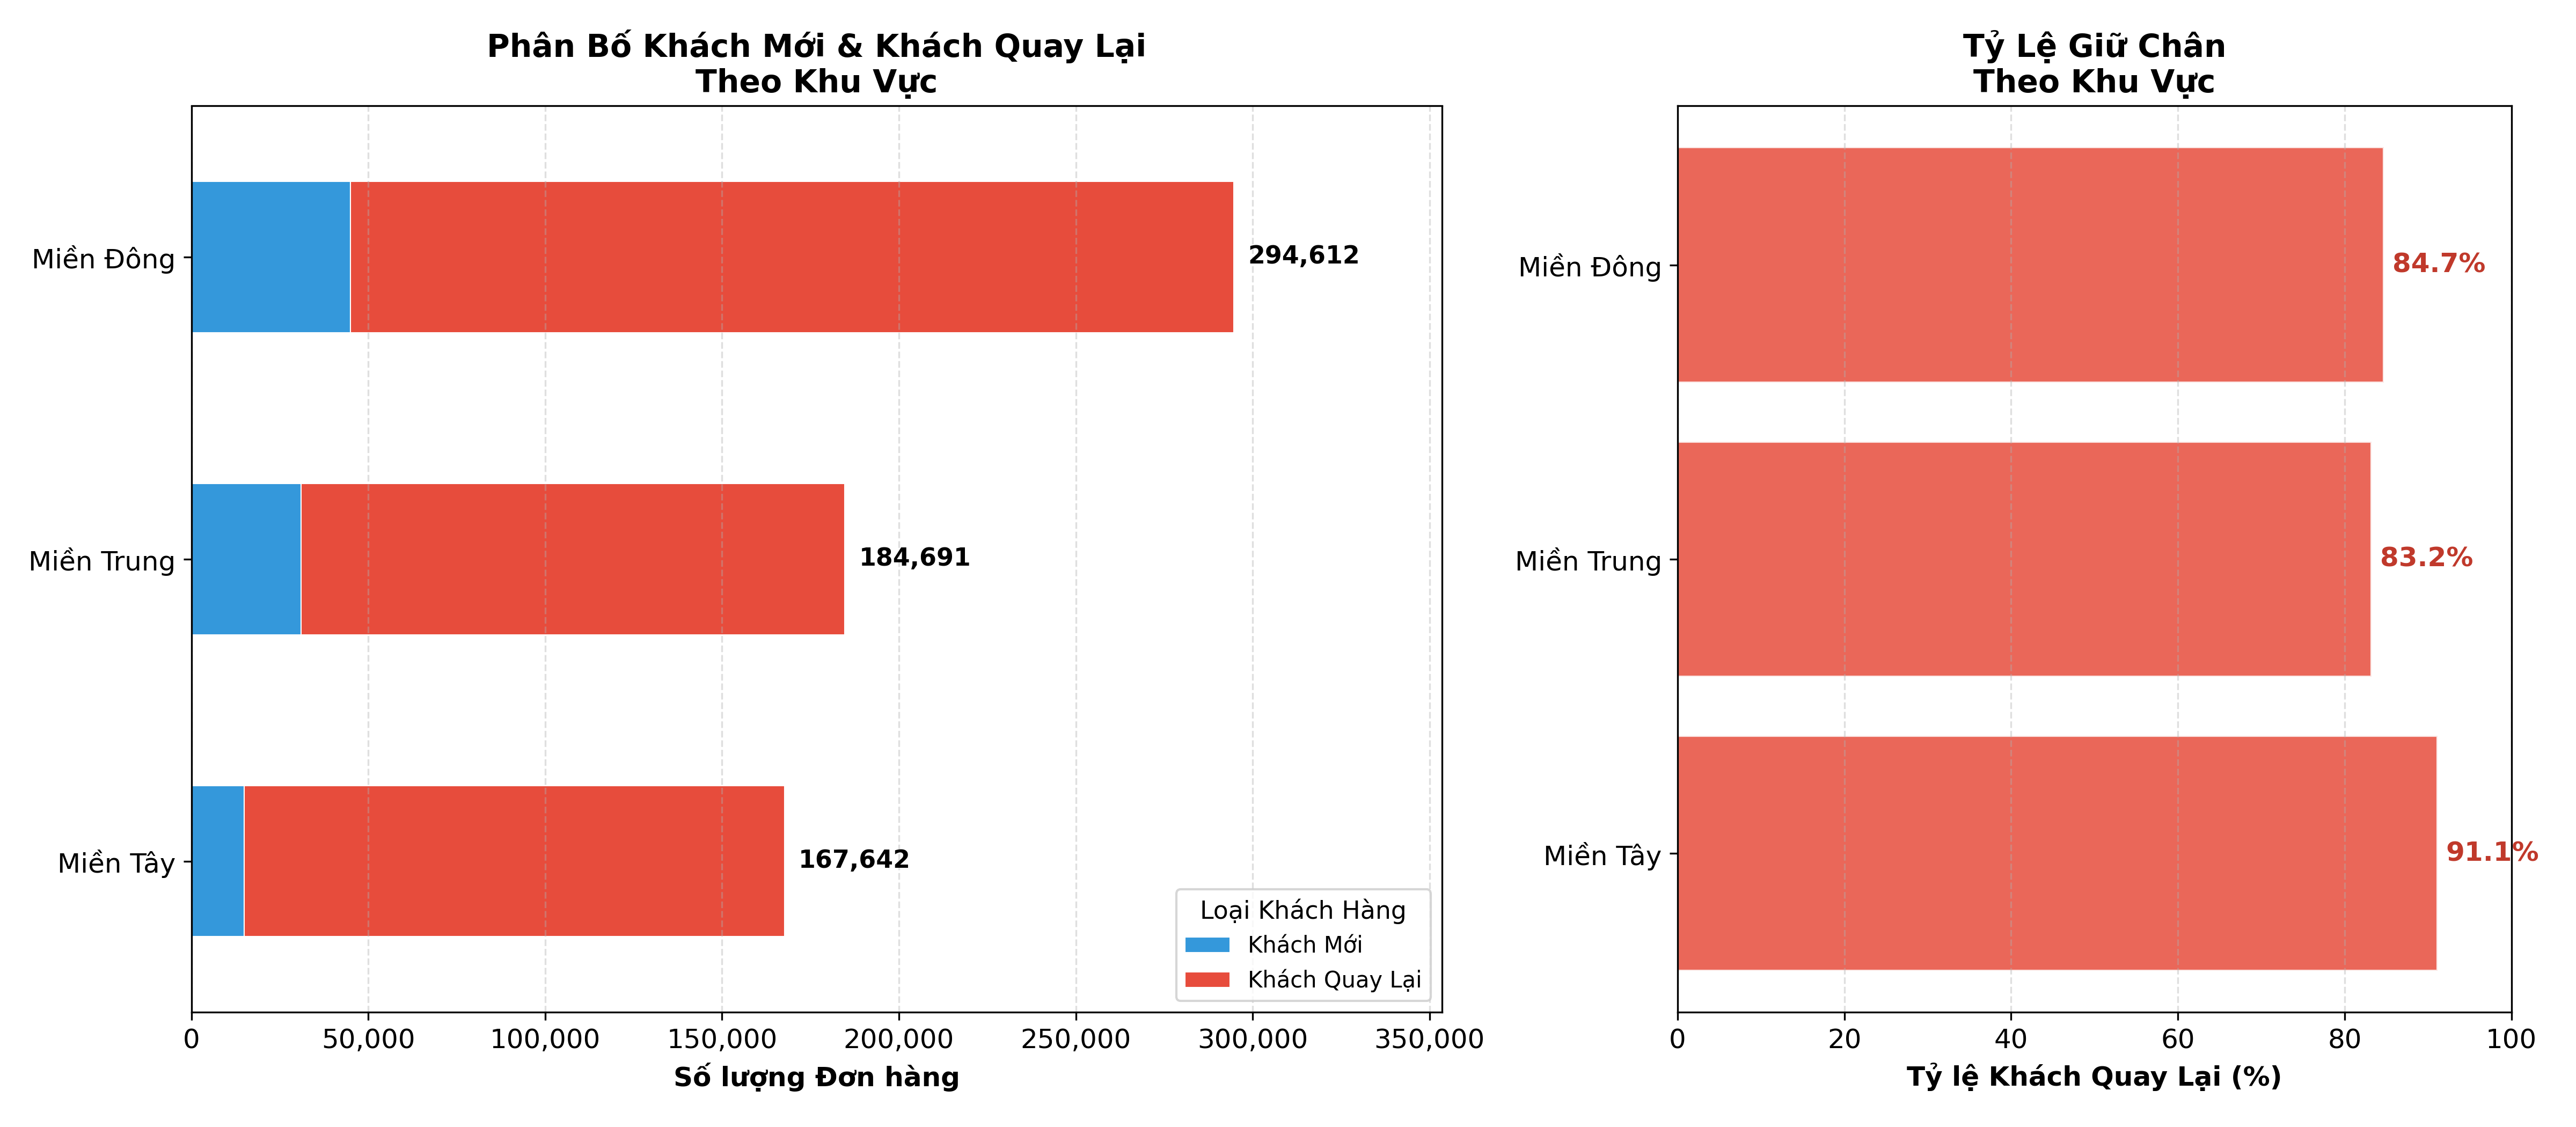
\includegraphics[width=0.48\textwidth]{Images/11a_Market_Penetration_Region.png}
    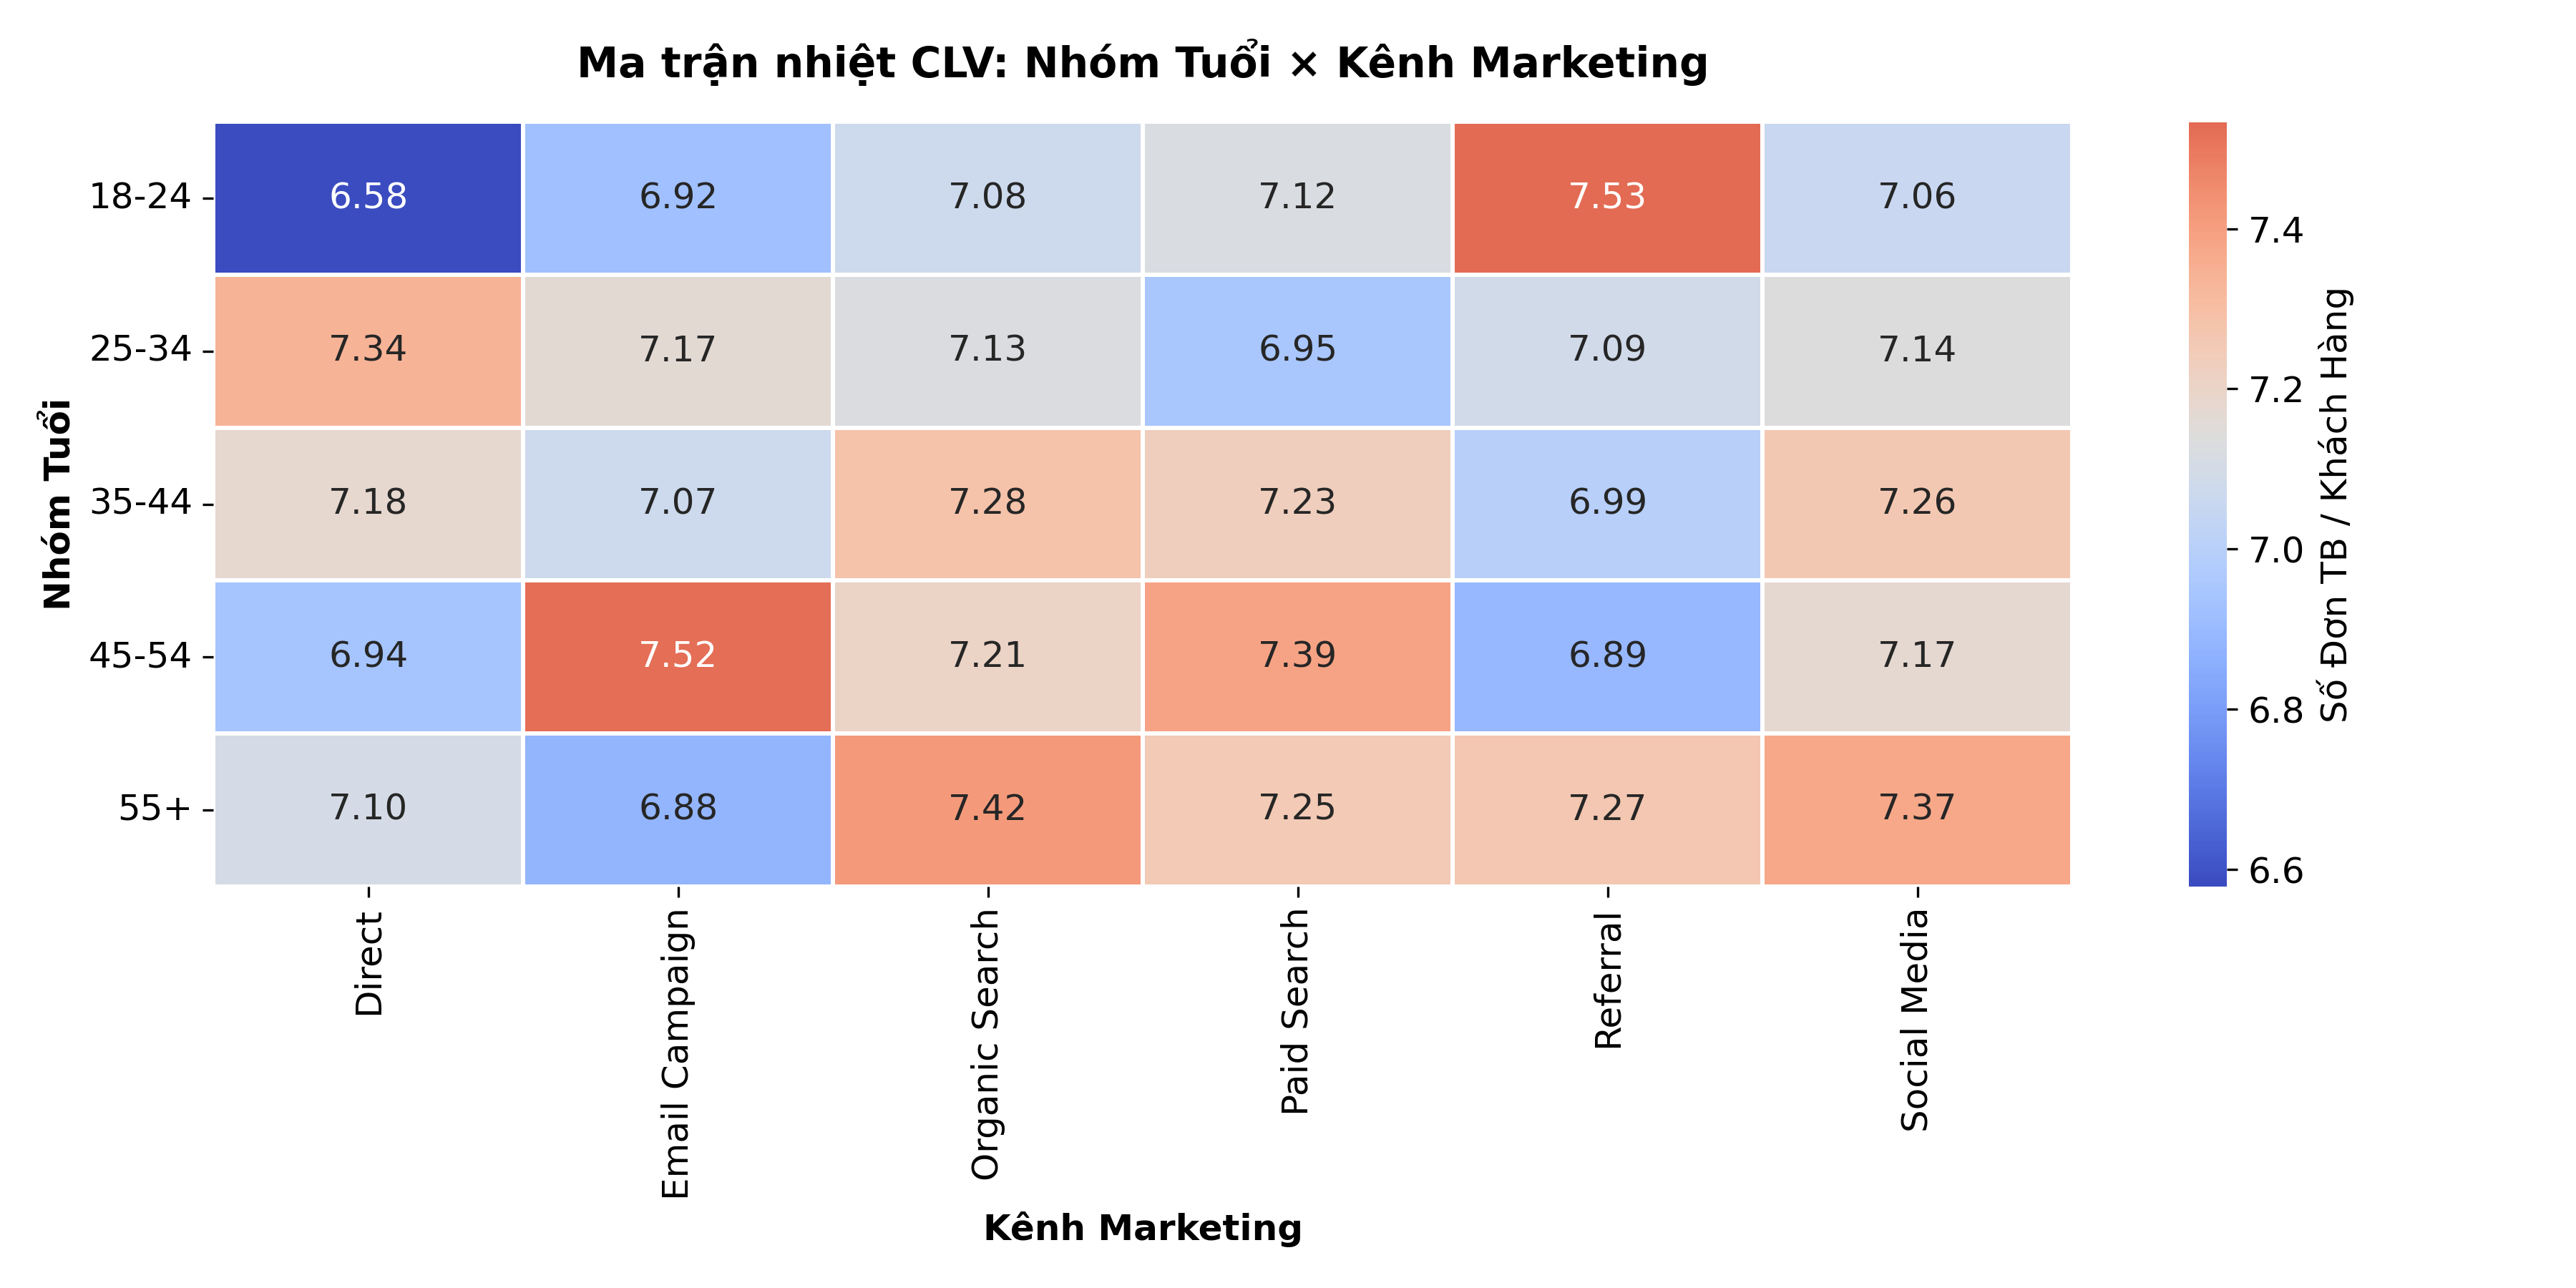
\includegraphics[width=0.48\textwidth]{Images/11c_CLV_Heatmap_Age_Channel.png}
    \caption{(Trái) Market Penetration theo khu vực. (Phải) CLV Heatmap: Nhóm Tuổi $\times$ Kênh Marketing.}
    \label{fig:appendix3}
\end{figure}

\end{document}
